% Options for packages loaded elsewhere
\PassOptionsToPackage{unicode}{hyperref}
\PassOptionsToPackage{hyphens}{url}
\PassOptionsToPackage{dvipsnames,svgnames,x11names}{xcolor}
%
\documentclass[
  11pt,
]{article}

\usepackage{amsmath,amssymb}
\usepackage{iftex}
\ifPDFTeX
  \usepackage[T1]{fontenc}
  \usepackage[utf8]{inputenc}
  \usepackage{textcomp} % provide euro and other symbols
\else % if luatex or xetex
  \usepackage{unicode-math}
  \defaultfontfeatures{Scale=MatchLowercase}
  \defaultfontfeatures[\rmfamily]{Ligatures=TeX,Scale=1}
\fi
\usepackage{lmodern}
\ifPDFTeX\else  
    % xetex/luatex font selection
\fi
% Use upquote if available, for straight quotes in verbatim environments
\IfFileExists{upquote.sty}{\usepackage{upquote}}{}
\IfFileExists{microtype.sty}{% use microtype if available
  \usepackage[]{microtype}
  \UseMicrotypeSet[protrusion]{basicmath} % disable protrusion for tt fonts
}{}
\makeatletter
\@ifundefined{KOMAClassName}{% if non-KOMA class
  \IfFileExists{parskip.sty}{%
    \usepackage{parskip}
  }{% else
    \setlength{\parindent}{0pt}
    \setlength{\parskip}{6pt plus 2pt minus 1pt}}
}{% if KOMA class
  \KOMAoptions{parskip=half}}
\makeatother
\usepackage{xcolor}
\ifLuaTeX
  \usepackage{luacolor}
  \usepackage[soul]{lua-ul}
\else
  \usepackage{soul}
  
\fi
\setlength{\emergencystretch}{3em} % prevent overfull lines
\setcounter{secnumdepth}{-\maxdimen} % remove section numbering
% Make \paragraph and \subparagraph free-standing
\makeatletter
\ifx\paragraph\undefined\else
  \let\oldparagraph\paragraph
  \renewcommand{\paragraph}{
    \@ifstar
      \xxxParagraphStar
      \xxxParagraphNoStar
  }
  \newcommand{\xxxParagraphStar}[1]{\oldparagraph*{#1}\mbox{}}
  \newcommand{\xxxParagraphNoStar}[1]{\oldparagraph{#1}\mbox{}}
\fi
\ifx\subparagraph\undefined\else
  \let\oldsubparagraph\subparagraph
  \renewcommand{\subparagraph}{
    \@ifstar
      \xxxSubParagraphStar
      \xxxSubParagraphNoStar
  }
  \newcommand{\xxxSubParagraphStar}[1]{\oldsubparagraph*{#1}\mbox{}}
  \newcommand{\xxxSubParagraphNoStar}[1]{\oldsubparagraph{#1}\mbox{}}
\fi
\makeatother

\usepackage{color}
\usepackage{fancyvrb}
\newcommand{\VerbBar}{|}
\newcommand{\VERB}{\Verb[commandchars=\\\{\}]}
\DefineVerbatimEnvironment{Highlighting}{Verbatim}{commandchars=\\\{\}}
% Add ',fontsize=\small' for more characters per line
\usepackage{framed}
\definecolor{shadecolor}{RGB}{241,243,245}
\newenvironment{Shaded}{\begin{snugshade}}{\end{snugshade}}
\newcommand{\AlertTok}[1]{\textcolor[rgb]{0.68,0.00,0.00}{#1}}
\newcommand{\AnnotationTok}[1]{\textcolor[rgb]{0.37,0.37,0.37}{#1}}
\newcommand{\AttributeTok}[1]{\textcolor[rgb]{0.40,0.45,0.13}{#1}}
\newcommand{\BaseNTok}[1]{\textcolor[rgb]{0.68,0.00,0.00}{#1}}
\newcommand{\BuiltInTok}[1]{\textcolor[rgb]{0.00,0.23,0.31}{#1}}
\newcommand{\CharTok}[1]{\textcolor[rgb]{0.13,0.47,0.30}{#1}}
\newcommand{\CommentTok}[1]{\textcolor[rgb]{0.37,0.37,0.37}{#1}}
\newcommand{\CommentVarTok}[1]{\textcolor[rgb]{0.37,0.37,0.37}{\textit{#1}}}
\newcommand{\ConstantTok}[1]{\textcolor[rgb]{0.56,0.35,0.01}{#1}}
\newcommand{\ControlFlowTok}[1]{\textcolor[rgb]{0.00,0.23,0.31}{\textbf{#1}}}
\newcommand{\DataTypeTok}[1]{\textcolor[rgb]{0.68,0.00,0.00}{#1}}
\newcommand{\DecValTok}[1]{\textcolor[rgb]{0.68,0.00,0.00}{#1}}
\newcommand{\DocumentationTok}[1]{\textcolor[rgb]{0.37,0.37,0.37}{\textit{#1}}}
\newcommand{\ErrorTok}[1]{\textcolor[rgb]{0.68,0.00,0.00}{#1}}
\newcommand{\ExtensionTok}[1]{\textcolor[rgb]{0.00,0.23,0.31}{#1}}
\newcommand{\FloatTok}[1]{\textcolor[rgb]{0.68,0.00,0.00}{#1}}
\newcommand{\FunctionTok}[1]{\textcolor[rgb]{0.28,0.35,0.67}{#1}}
\newcommand{\ImportTok}[1]{\textcolor[rgb]{0.00,0.46,0.62}{#1}}
\newcommand{\InformationTok}[1]{\textcolor[rgb]{0.37,0.37,0.37}{#1}}
\newcommand{\KeywordTok}[1]{\textcolor[rgb]{0.00,0.23,0.31}{\textbf{#1}}}
\newcommand{\NormalTok}[1]{\textcolor[rgb]{0.00,0.23,0.31}{#1}}
\newcommand{\OperatorTok}[1]{\textcolor[rgb]{0.37,0.37,0.37}{#1}}
\newcommand{\OtherTok}[1]{\textcolor[rgb]{0.00,0.23,0.31}{#1}}
\newcommand{\PreprocessorTok}[1]{\textcolor[rgb]{0.68,0.00,0.00}{#1}}
\newcommand{\RegionMarkerTok}[1]{\textcolor[rgb]{0.00,0.23,0.31}{#1}}
\newcommand{\SpecialCharTok}[1]{\textcolor[rgb]{0.37,0.37,0.37}{#1}}
\newcommand{\SpecialStringTok}[1]{\textcolor[rgb]{0.13,0.47,0.30}{#1}}
\newcommand{\StringTok}[1]{\textcolor[rgb]{0.13,0.47,0.30}{#1}}
\newcommand{\VariableTok}[1]{\textcolor[rgb]{0.07,0.07,0.07}{#1}}
\newcommand{\VerbatimStringTok}[1]{\textcolor[rgb]{0.13,0.47,0.30}{#1}}
\newcommand{\WarningTok}[1]{\textcolor[rgb]{0.37,0.37,0.37}{\textit{#1}}}

\providecommand{\tightlist}{%
  \setlength{\itemsep}{0pt}\setlength{\parskip}{0pt}}\usepackage{longtable,booktabs,array}
\usepackage{calc} % for calculating minipage widths
% Correct order of tables after \paragraph or \subparagraph
\usepackage{etoolbox}
\makeatletter
\patchcmd\longtable{\par}{\if@noskipsec\mbox{}\fi\par}{}{}
\makeatother
% Allow footnotes in longtable head/foot
\IfFileExists{footnotehyper.sty}{\usepackage{footnotehyper}}{\usepackage{footnote}}
\makesavenoteenv{longtable}
\usepackage{graphicx}
\makeatletter
\def\maxwidth{\ifdim\Gin@nat@width>\linewidth\linewidth\else\Gin@nat@width\fi}
\def\maxheight{\ifdim\Gin@nat@height>\textheight\textheight\else\Gin@nat@height\fi}
\makeatother
% Scale images if necessary, so that they will not overflow the page
% margins by default, and it is still possible to overwrite the defaults
% using explicit options in \includegraphics[width, height, ...]{}
\setkeys{Gin}{width=\maxwidth,height=\maxheight,keepaspectratio}
% Set default figure placement to htbp
\makeatletter
\def\fps@figure{htbp}
\makeatother

\usepackage{setspace}
\setstretch{1.1}
\usepackage{geometry}
\geometry{margin=0.7in}
\usepackage{parskip}
\setlength{\parskip}{0.5em}
\setlength{\parindent}{0.4em}
\usepackage{listings}
\lstset{breaklines=true, basicstyle=\footnotesize\ttfamily, linewidth=\textwidth, frame=single}
\usepackage{graphicx}
\usepackage{longtable}
\usepackage{caption}
\captionsetup{width=\textwidth}
\usepackage{mathptmx}
\usepackage{mdframed}
\mdfdefinestyle{boxedoutputstyle}{linewidth=1pt, roundcorner=5pt}
\makeatletter
\@ifpackageloaded{caption}{}{\usepackage{caption}}
\AtBeginDocument{%
\ifdefined\contentsname
  \renewcommand*\contentsname{Table of contents}
\else
  \newcommand\contentsname{Table of contents}
\fi
\ifdefined\listfigurename
  \renewcommand*\listfigurename{List of Figures}
\else
  \newcommand\listfigurename{List of Figures}
\fi
\ifdefined\listtablename
  \renewcommand*\listtablename{List of Tables}
\else
  \newcommand\listtablename{List of Tables}
\fi
\ifdefined\figurename
  \renewcommand*\figurename{Figure}
\else
  \newcommand\figurename{Figure}
\fi
\ifdefined\tablename
  \renewcommand*\tablename{Table}
\else
  \newcommand\tablename{Table}
\fi
}
\@ifpackageloaded{float}{}{\usepackage{float}}
\floatstyle{ruled}
\@ifundefined{c@chapter}{\newfloat{codelisting}{h}{lop}}{\newfloat{codelisting}{h}{lop}[chapter]}
\floatname{codelisting}{Listing}
\newcommand*\listoflistings{\listof{codelisting}{List of Listings}}
\makeatother
\makeatletter
\makeatother
\makeatletter
\@ifpackageloaded{caption}{}{\usepackage{caption}}
\@ifpackageloaded{subcaption}{}{\usepackage{subcaption}}
\makeatother

\ifLuaTeX
  \usepackage{selnolig}  % disable illegal ligatures
\fi
\usepackage{bookmark}

\IfFileExists{xurl.sty}{\usepackage{xurl}}{} % add URL line breaks if available
\urlstyle{same} % disable monospaced font for URLs
\hypersetup{
  pdftitle={HW-4},
  colorlinks=true,
  linkcolor={blue},
  filecolor={Maroon},
  citecolor={Blue},
  urlcolor={Blue},
  pdfcreator={LaTeX via pandoc}}


\title{HW-4}
\author{}
\date{}

\begin{document}
\maketitle


\subsection{STATS 500 - HOMEWORK 4}\label{stats-500---homework-4}

\subsection{Vasudha Rohatgi}\label{vasudha-rohatgi}

Code Published at \url{https://github.com/Vasu2499/STATS-500-HW-4}

\subsubsection{PROBLEM 1}\label{problem-1}

\paragraph{\texorpdfstring{\ul{\textbf{PART
(a)}}}{PART (a)}}\label{part-a}

\begin{Shaded}
\begin{Highlighting}[]
\CommentTok{\# install.packages("car")}
\CommentTok{\# install.packages("lmtest")}
\FunctionTok{library}\NormalTok{(car)}
\end{Highlighting}
\end{Shaded}

\begin{verbatim}
Loading required package: carData
\end{verbatim}

\begin{Shaded}
\begin{Highlighting}[]
\FunctionTok{library}\NormalTok{(lmtest)}
\end{Highlighting}
\end{Shaded}

\begin{verbatim}
Loading required package: zoo
\end{verbatim}

\begin{verbatim}

Attaching package: 'zoo'
\end{verbatim}

\begin{verbatim}
The following objects are masked from 'package:base':

    as.Date, as.Date.numeric
\end{verbatim}

\begin{Shaded}
\begin{Highlighting}[]
\FunctionTok{library}\NormalTok{(broom)}
\FunctionTok{library}\NormalTok{(ggplot2)}


\DocumentationTok{\#\# I created both vectors manually to avoid errors }
\DocumentationTok{\#\# related to data loading/type mismatch }

\NormalTok{DATA\_X\_Y }\OtherTok{\textless{}{-}} \FunctionTok{data.frame}\NormalTok{(}
  \AttributeTok{x =} \FunctionTok{c}\NormalTok{(}\FloatTok{0.172038167}\NormalTok{, }\FloatTok{0.418466777}\NormalTok{, }\FloatTok{0.054523322}\NormalTok{, }\FloatTok{0.695505929}\NormalTok{, }\FloatTok{0.980692884}\NormalTok{, }\FloatTok{0.607070161}\NormalTok{, }
        \FloatTok{0.011947568}\NormalTok{, }\FloatTok{0.435136626}\NormalTok{, }\FloatTok{0.894557753}\NormalTok{, }\FloatTok{0.83386622}\NormalTok{, }\FloatTok{0.281672534}\NormalTok{, }\FloatTok{0.33573479}\NormalTok{, }
        \FloatTok{0.045642636}\NormalTok{, }\FloatTok{0.8848521}\NormalTok{, }\FloatTok{0.96812355}\NormalTok{, }\FloatTok{0.571297675}\NormalTok{, }\FloatTok{0.716719676}\NormalTok{, }\FloatTok{0.07434831}\NormalTok{, }
        \FloatTok{0.265655909}\NormalTok{, }\FloatTok{0.170830833}\NormalTok{, }\FloatTok{0.724962878}\NormalTok{, }\FloatTok{0.421258879}\NormalTok{, }\FloatTok{0.04217659}\NormalTok{, }\FloatTok{0.619995055}\NormalTok{, }
        \FloatTok{0.765302866}\NormalTok{, }\FloatTok{0.715242532}\NormalTok{, }\FloatTok{0.784955135}\NormalTok{, }\FloatTok{0.272284389}\NormalTok{, }\FloatTok{0.026605156}\NormalTok{, }\FloatTok{0.986976457}\NormalTok{, }
        \FloatTok{0.058915448}\NormalTok{, }\FloatTok{0.559899994}\NormalTok{, }\FloatTok{0.149852436}\NormalTok{, }\FloatTok{0.372403622}\NormalTok{, }\FloatTok{0.295098473}\NormalTok{, }\FloatTok{0.197134535}\NormalTok{, }
        \FloatTok{0.695133297}\NormalTok{, }\FloatTok{0.742518261}\NormalTok{, }\FloatTok{0.825313237}\NormalTok{, }\FloatTok{0.484748986}\NormalTok{, }\FloatTok{0.675808315}\NormalTok{, }\FloatTok{0.7916749}\NormalTok{, }
        \FloatTok{0.355265427}\NormalTok{, }\FloatTok{0.044775931}\NormalTok{, }\FloatTok{0.169300308}\NormalTok{, }\FloatTok{0.795860181}\NormalTok{, }\FloatTok{0.733278047}\NormalTok{, }\FloatTok{0.569696626}\NormalTok{, }
        \FloatTok{0.342122064}\NormalTok{, }\FloatTok{0.482784098}\NormalTok{, }\FloatTok{0.257727252}\NormalTok{, }\FloatTok{0.992103707}\NormalTok{, }\FloatTok{0.353837485}\NormalTok{, }\FloatTok{0.402662357}\NormalTok{, }
        \FloatTok{0.303802435}\NormalTok{, }\FloatTok{0.25241684}\NormalTok{, }\FloatTok{0.404298493}\NormalTok{, }\FloatTok{0.221529326}\NormalTok{, }\FloatTok{0.259792642}\NormalTok{, }\FloatTok{0.234567108}\NormalTok{, }
        \FloatTok{0.878760028}\NormalTok{, }\FloatTok{0.024527291}\NormalTok{, }\FloatTok{0.497956215}\NormalTok{, }\FloatTok{0.693973705}\NormalTok{, }\FloatTok{0.502646435}\NormalTok{, }\FloatTok{0.51743757}\NormalTok{, }
        \FloatTok{0.334757277}\NormalTok{, }\FloatTok{0.018371782}\NormalTok{, }\FloatTok{0.844523574}\NormalTok{, }\FloatTok{0.356896266}\NormalTok{, }\FloatTok{0.212493253}\NormalTok{, }\FloatTok{0.296758583}\NormalTok{, }
        \FloatTok{0.474448235}\NormalTok{, }\FloatTok{0.771659764}\NormalTok{, }\FloatTok{0.872904745}\NormalTok{, }\FloatTok{0.069980517}\NormalTok{, }\FloatTok{0.16414597}\NormalTok{, }\FloatTok{0.137929959}\NormalTok{, }
        \FloatTok{0.442823663}\NormalTok{, }\FloatTok{0.53376598}\NormalTok{, }\FloatTok{0.755756296}\NormalTok{, }\FloatTok{0.855570187}\NormalTok{, }\FloatTok{0.699383936}\NormalTok{, }\FloatTok{0.907087586}\NormalTok{, }
        \FloatTok{0.805959126}\NormalTok{, }\FloatTok{0.388349324}\NormalTok{, }\FloatTok{0.195891048}\NormalTok{, }\FloatTok{0.601747278}\NormalTok{, }\FloatTok{0.469033639}\NormalTok{, }\FloatTok{0.453257746}\NormalTok{, }
        \FloatTok{0.537691873}\NormalTok{, }\FloatTok{0.299450343}\NormalTok{, }\FloatTok{0.476787878}\NormalTok{, }\FloatTok{0.569891095}\NormalTok{, }\FloatTok{0.114090955}\NormalTok{, }\FloatTok{0.756277627}\NormalTok{, }
        \FloatTok{0.484390114}\NormalTok{, }\FloatTok{0.866153744}\NormalTok{, }\FloatTok{0.838347831}\NormalTok{, }\FloatTok{0.423012322}\NormalTok{),}
  \AttributeTok{y =} \FunctionTok{c}\NormalTok{(}\FloatTok{0.615463909}\NormalTok{, }\FloatTok{2.786868902}\NormalTok{, }\FloatTok{1.391114421}\NormalTok{, }\FloatTok{5.513140781}\NormalTok{, }\FloatTok{8.928013838}\NormalTok{, }\FloatTok{4.068108402}\NormalTok{,}
        \FloatTok{0.063691378}\NormalTok{, }\FloatTok{3.110613949}\NormalTok{, }\FloatTok{4.511442248}\NormalTok{, }\FloatTok{5.888070504}\NormalTok{, }\FloatTok{4.311799621}\NormalTok{, }\FloatTok{2.764826737}\NormalTok{,}
        \SpecialCharTok{{-}}\FloatTok{0.892588409}\NormalTok{, }\FloatTok{12.75371213}\NormalTok{, }\FloatTok{4.528309356}\NormalTok{, }\FloatTok{3.595944921}\NormalTok{, }\FloatTok{3.609635666}\NormalTok{, }\FloatTok{1.76275869}\NormalTok{,}
        \FloatTok{3.147503883}\NormalTok{, }\FloatTok{1.456565682}\NormalTok{, }\FloatTok{3.93219418}\NormalTok{, }\FloatTok{2.972703801}\NormalTok{, }\FloatTok{0.873412578}\NormalTok{, }\FloatTok{3.984062378}\NormalTok{,}
        \FloatTok{4.949698937}\NormalTok{, }\FloatTok{7.131532014}\NormalTok{, }\FloatTok{7.079722233}\NormalTok{, }\FloatTok{11.86116384}\NormalTok{, }\FloatTok{0.244303005}\NormalTok{, }\FloatTok{3.692677683}\NormalTok{,}
        \FloatTok{2.147189199}\NormalTok{, }\FloatTok{3.605006326}\NormalTok{, }\FloatTok{1.032537933}\NormalTok{, }\FloatTok{2.655585392}\NormalTok{, }\FloatTok{1.656532377}\NormalTok{, }\FloatTok{3.404987867}\NormalTok{,}
        \FloatTok{3.701615913}\NormalTok{, }\FloatTok{10.27326537}\NormalTok{, }\FloatTok{7.169696402}\NormalTok{, }\FloatTok{3.585939694}\NormalTok{, }\FloatTok{6.043443262}\NormalTok{, }\FloatTok{3.455010225}\NormalTok{,}
        \FloatTok{2.476542828}\NormalTok{, }\FloatTok{5.997966752}\NormalTok{, }\FloatTok{0.75690345}\NormalTok{, }\FloatTok{4.276901278}\NormalTok{, }\FloatTok{3.597403681}\NormalTok{, }\FloatTok{3.648705215}\NormalTok{,}
        \FloatTok{1.998482562}\NormalTok{, }\FloatTok{3.460836761}\NormalTok{, }\FloatTok{1.81163011}\NormalTok{, }\FloatTok{3.672050336}\NormalTok{, }\FloatTok{4.563573561}\NormalTok{, }\FloatTok{2.947486015}\NormalTok{,}
        \FloatTok{3.671598776}\NormalTok{, }\FloatTok{1.079755993}\NormalTok{, }\FloatTok{4.014472991}\NormalTok{, }\FloatTok{0.803146673}\NormalTok{, }\FloatTok{1.636552647}\NormalTok{, }\FloatTok{1.488315055}\NormalTok{,}
        \FloatTok{9.048456133}\NormalTok{, }\FloatTok{0.059128936}\NormalTok{, }\FloatTok{3.483556904}\NormalTok{, }\FloatTok{3.63638176}\NormalTok{, }\FloatTok{3.505882982}\NormalTok{, }\FloatTok{3.554139102}\NormalTok{,}
        \FloatTok{1.916388836}\NormalTok{, }\FloatTok{2.152735695}\NormalTok{, }\FloatTok{5.154818385}\NormalTok{, }\FloatTok{2.645536336}\NormalTok{, }\FloatTok{1.280925658}\NormalTok{, }\FloatTok{1.688439264}\NormalTok{,}
        \FloatTok{3.256380613}\NormalTok{, }\FloatTok{4.33833951}\NormalTok{, }\FloatTok{3.877387878}\NormalTok{, }\FloatTok{1.397218401}\NormalTok{, }\FloatTok{2.402945759}\NormalTok{, }\FloatTok{3.980154753}\NormalTok{,}
        \FloatTok{2.93424781}\NormalTok{, }\FloatTok{3.59075253}\NormalTok{, }\FloatTok{4.094248288}\NormalTok{, }\FloatTok{7.796327544}\NormalTok{, }\FloatTok{3.890117281}\NormalTok{, }\FloatTok{3.718084517}\NormalTok{,}
        \FloatTok{4.400256847}\NormalTok{, }\FloatTok{2.431933865}\NormalTok{, }\FloatTok{2.998349391}\NormalTok{, }\FloatTok{3.934755336}\NormalTok{, }\FloatTok{3.446353977}\NormalTok{, }\FloatTok{3.542439376}\NormalTok{,}
        \FloatTok{3.52940814}\NormalTok{, }\FloatTok{6.278667985}\NormalTok{, }\FloatTok{3.289264874}\NormalTok{, }\FloatTok{3.793658899}\NormalTok{, }\FloatTok{3.998930738}\NormalTok{, }\FloatTok{4.583571992}\NormalTok{,}
        \FloatTok{3.392036397}\NormalTok{, }\FloatTok{5.292731256}\NormalTok{, }\FloatTok{4.880063631}\NormalTok{, }\FloatTok{3.127386419}\NormalTok{)}
\NormalTok{)}


\CommentTok{\# Fit linear model}
\NormalTok{model }\OtherTok{\textless{}{-}} \FunctionTok{lm}\NormalTok{(y }\SpecialCharTok{\textasciitilde{}}\NormalTok{ x, }\AttributeTok{data =}\NormalTok{ DATA\_X\_Y)}

\CommentTok{\# Summary of the model}
\FunctionTok{summary}\NormalTok{(model)}
\end{Highlighting}
\end{Shaded}

\begin{verbatim}

Call:
lm(formula = y ~ x, data = DATA_X_Y)

Residuals:
    Min      1Q  Median      3Q     Max 
-2.5499 -0.9772 -0.3922  0.3329  9.2143 

Coefficients:
            Estimate Std. Error t value Pr(>|t|)    
(Intercept)   1.2945     0.3627   3.569 0.000558 ***
x             4.9667     0.6543   7.591 1.88e-11 ***
---
Signif. codes:  0 '***' 0.001 '**' 0.01 '*' 0.05 '.' 0.1 ' ' 1

Residual standard error: 1.821 on 98 degrees of freedom
Multiple R-squared:  0.3703,    Adjusted R-squared:  0.3638 
F-statistic: 57.62 on 1 and 98 DF,  p-value: 1.875e-11
\end{verbatim}

\begin{Shaded}
\begin{Highlighting}[]
\CommentTok{\# Diagnostic plots}

\NormalTok{diagnostics }\OtherTok{\textless{}{-}} \FunctionTok{augment}\NormalTok{(model)}

\CommentTok{\# Residuals vs. Fitted}
\FunctionTok{ggplot}\NormalTok{(diagnostics, }\FunctionTok{aes}\NormalTok{(.fitted, .resid)) }\SpecialCharTok{+}
  \FunctionTok{geom\_point}\NormalTok{(}\AttributeTok{color =} \StringTok{"navy"}\NormalTok{, }\AttributeTok{alpha =} \FloatTok{0.8}\NormalTok{) }\SpecialCharTok{+}
  \FunctionTok{geom\_hline}\NormalTok{(}\AttributeTok{yintercept =} \DecValTok{0}\NormalTok{, }\AttributeTok{linetype =} \StringTok{"dashed"}\NormalTok{) }\SpecialCharTok{+}
  \FunctionTok{labs}\NormalTok{(}\AttributeTok{title =} \StringTok{"Residuals vs Fitted"}\NormalTok{, }\AttributeTok{x =} \StringTok{"Fitted values"}\NormalTok{, }
       \AttributeTok{y =} \StringTok{"Residuals"}\NormalTok{) }\SpecialCharTok{+}
  \FunctionTok{theme\_minimal}\NormalTok{()}
\end{Highlighting}
\end{Shaded}

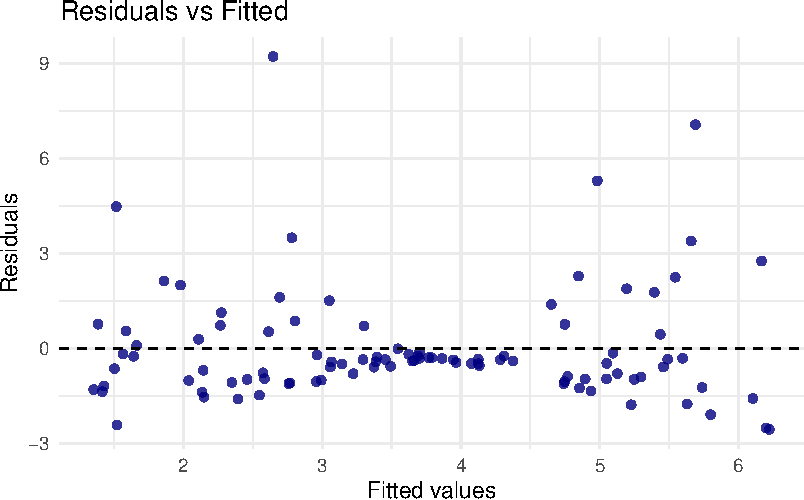
\includegraphics{HW-4-CODE-and-ANSWERS_files/figure-pdf/unnamed-chunk-1-1.pdf}

\begin{Shaded}
\begin{Highlighting}[]
\CommentTok{\# Normal Q{-}Q}
\FunctionTok{ggplot}\NormalTok{(diagnostics, }\FunctionTok{aes}\NormalTok{(}\AttributeTok{sample =}\NormalTok{ .std.resid)) }\SpecialCharTok{+}
  \FunctionTok{stat\_qq}\NormalTok{(}\AttributeTok{color =} \StringTok{"navy"}\NormalTok{) }\SpecialCharTok{+}
  \FunctionTok{stat\_qq\_line}\NormalTok{(}\AttributeTok{color =} \StringTok{"darkred"}\NormalTok{) }\SpecialCharTok{+}
  \FunctionTok{labs}\NormalTok{(}\AttributeTok{title =} \StringTok{"Normal Q{-}Q"}\NormalTok{, }\AttributeTok{x =} \StringTok{"Theoretical Quantiles"}\NormalTok{, }
       \AttributeTok{y =} \StringTok{"Standardized Residuals"}\NormalTok{) }\SpecialCharTok{+}
  \FunctionTok{theme\_minimal}\NormalTok{()}
\end{Highlighting}
\end{Shaded}

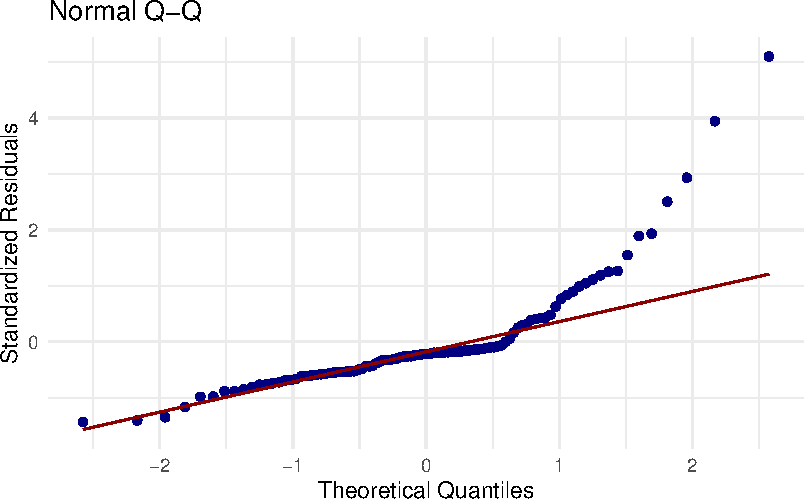
\includegraphics{HW-4-CODE-and-ANSWERS_files/figure-pdf/unnamed-chunk-2-1.pdf}

\begin{Shaded}
\begin{Highlighting}[]
\CommentTok{\# Scale{-}Location }
\FunctionTok{ggplot}\NormalTok{(diagnostics, }\FunctionTok{aes}\NormalTok{(.fitted, }\FunctionTok{sqrt}\NormalTok{(}\FunctionTok{abs}\NormalTok{(.std.resid)))) }\SpecialCharTok{+}
  \FunctionTok{geom\_point}\NormalTok{(}\AttributeTok{color =} \StringTok{"navy"}\NormalTok{, }\AttributeTok{alpha =} \FloatTok{0.8}\NormalTok{) }\SpecialCharTok{+}
  \FunctionTok{geom\_smooth}\NormalTok{(}\AttributeTok{se =} \ConstantTok{FALSE}\NormalTok{, }\AttributeTok{color =} \StringTok{"darkred"}\NormalTok{) }\SpecialCharTok{+}
  \FunctionTok{labs}\NormalTok{(}\AttributeTok{title =} \StringTok{"Scale{-}Location"}\NormalTok{, }\AttributeTok{x =} \StringTok{"Fitted values"}\NormalTok{, }
       \AttributeTok{y =} \StringTok{"Sqrt( | Standardized Residuals | )"}\NormalTok{) }\SpecialCharTok{+}
  \FunctionTok{theme\_minimal}\NormalTok{()}
\end{Highlighting}
\end{Shaded}

\begin{verbatim}
`geom_smooth()` using method = 'loess' and formula = 'y ~ x'
\end{verbatim}

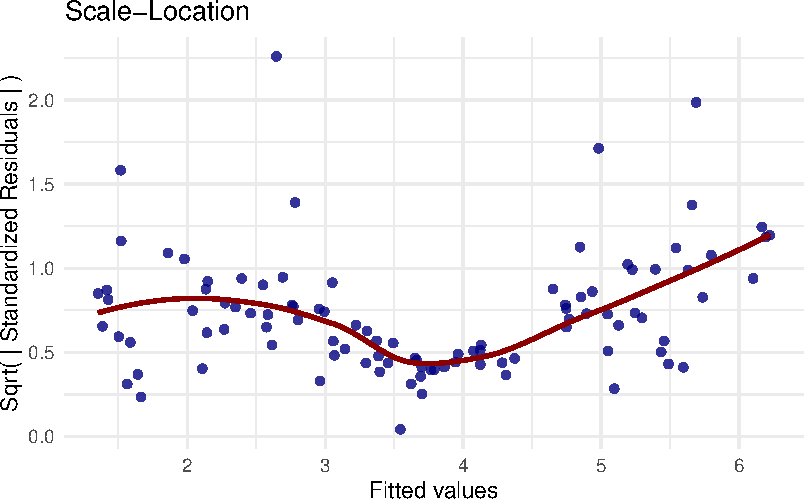
\includegraphics{HW-4-CODE-and-ANSWERS_files/figure-pdf/unnamed-chunk-3-1.pdf}

\begin{Shaded}
\begin{Highlighting}[]
\CommentTok{\# Residuals vs. Leverage}
\FunctionTok{ggplot}\NormalTok{(diagnostics, }\FunctionTok{aes}\NormalTok{(.hat, .std.resid)) }\SpecialCharTok{+}
  \FunctionTok{geom\_point}\NormalTok{(}\AttributeTok{color =} \StringTok{"navy"}\NormalTok{, }\AttributeTok{alpha =} \FloatTok{0.8}\NormalTok{) }\SpecialCharTok{+}
  \FunctionTok{geom\_smooth}\NormalTok{(}\AttributeTok{se =} \ConstantTok{FALSE}\NormalTok{, }\AttributeTok{color =} \StringTok{"darkred"}\NormalTok{) }\SpecialCharTok{+}
  \FunctionTok{labs}\NormalTok{(}\AttributeTok{title =} \StringTok{"Residuals vs Leverage"}\NormalTok{, }\AttributeTok{x =} \StringTok{"Leverage"}\NormalTok{, }
       \AttributeTok{y =} \StringTok{"Standardized Residuals"}\NormalTok{) }\SpecialCharTok{+}
  \FunctionTok{theme\_minimal}\NormalTok{()}
\end{Highlighting}
\end{Shaded}

\begin{verbatim}
`geom_smooth()` using method = 'loess' and formula = 'y ~ x'
\end{verbatim}

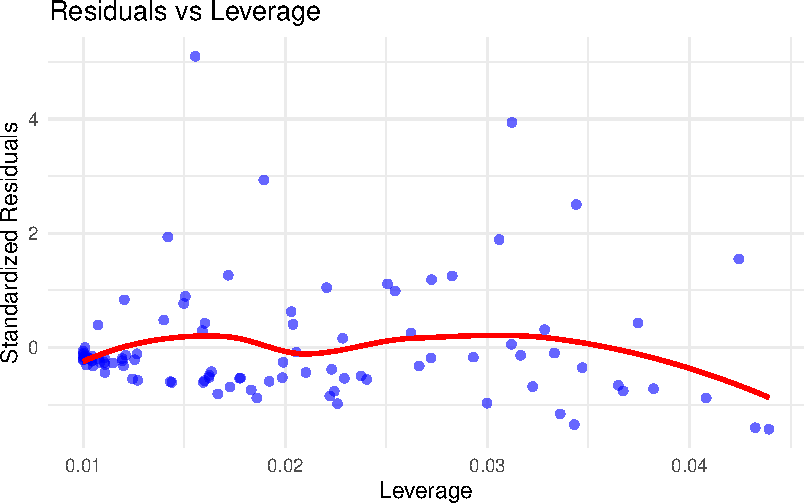
\includegraphics{HW-4-CODE-and-ANSWERS_files/figure-pdf/unnamed-chunk-4-1.pdf}

\paragraph{\texorpdfstring{\emph{Some
observations}}{Some observations}}\label{some-observations}

\begin{itemize}
\item
  \textbf{Residuals vs.~Fitted Plot}:

  \begin{itemize}
  \tightlist
  \item
    Mostly a straight line with slight deviations, indicating a mostly
    valid linear model with some mild non-linearity concerns.
  \end{itemize}
\item
  \textbf{Q-Q Plot}:

  \begin{itemize}
  \tightlist
  \item
    Resembles an exponential curve, suggesting non-normality of
    residuals, particularly right-skewed, which may affect inference.
  \end{itemize}
\item
  \textbf{Scale-Location Plot}:

  \begin{itemize}
  \tightlist
  \item
    Generally a straight horizontal line with a mild V-shape, indicating
    potential mild heteroskedasticity, which could lead to unreliable
    standard errors.
  \end{itemize}
\item
  \textbf{Residuals vs.~Leverage Plot}:

  \begin{itemize}
  \tightlist
  \item
    A dense cluster of points along a line with many outliers,
    indicating that while most points fit well, the outliers could
    significantly influence the regression results.
  \end{itemize}
\end{itemize}

\textbf{The model shows potential issues with non-normality and
heteroskedasticity, alongside influential outliers, which could
undermine the reliability of coefficient estimates and inference.}

\paragraph{\texorpdfstring{\ul{\textbf{PART (b) and
PART(c)}}}{PART (b) and PART(c)}}\label{part-b-and-partc}

\textsc{\emph{80\% Confidence Interval for the Slope Using Default
Standard Error}}\\
\textbf{\emph{(attached handwritten calculation)}}

\ul{\textbf{NEXT SEGMENT OF PROBLEM - 1 : DATA GENERATION}}

\begin{Shaded}
\begin{Highlighting}[]
\FunctionTok{set.seed}\NormalTok{(}\DecValTok{123}\NormalTok{)}
\NormalTok{n }\OtherTok{\textless{}{-}} \DecValTok{100}
\NormalTok{B }\OtherTok{\textless{}{-}} \DecValTok{10000}
\NormalTok{x }\OtherTok{\textless{}{-}}\NormalTok{ DATA\_X\_Y}\SpecialCharTok{$}\NormalTok{x}
\NormalTok{results }\OtherTok{\textless{}{-}} \FunctionTok{numeric}\NormalTok{(B)}

\ControlFlowTok{for}\NormalTok{ (b }\ControlFlowTok{in} \DecValTok{1}\SpecialCharTok{:}\NormalTok{B) \{}
\NormalTok{  epsilon }\OtherTok{\textless{}{-}} \FunctionTok{rnorm}\NormalTok{(n, }\AttributeTok{mean =} \DecValTok{0}\NormalTok{, }\AttributeTok{sd =} \FunctionTok{sqrt}\NormalTok{(}\FloatTok{0.75}\NormalTok{)) }
\NormalTok{  y }\OtherTok{\textless{}{-}} \DecValTok{1} \SpecialCharTok{+} \DecValTok{5} \SpecialCharTok{*}\NormalTok{ x }\SpecialCharTok{+}\NormalTok{ epsilon }
\NormalTok{  model }\OtherTok{\textless{}{-}} \FunctionTok{lm}\NormalTok{(y }\SpecialCharTok{\textasciitilde{}}\NormalTok{ x) }
\NormalTok{  results[b] }\OtherTok{\textless{}{-}} \FunctionTok{coef}\NormalTok{(model)[}\DecValTok{2}\NormalTok{] }
\NormalTok{\}}

\CommentTok{\# Calculating the coverage of the 80\% CI}
\NormalTok{lower\_bound }\OtherTok{\textless{}{-}} \FunctionTok{quantile}\NormalTok{(results, }\FloatTok{0.1}\NormalTok{)}
\NormalTok{upper\_bound }\OtherTok{\textless{}{-}} \FunctionTok{quantile}\NormalTok{(results, }\FloatTok{0.9}\NormalTok{)}
\NormalTok{coverage }\OtherTok{\textless{}{-}} \FunctionTok{mean}\NormalTok{((lower\_bound }\SpecialCharTok{\textless{}=} \DecValTok{5}\NormalTok{) }\SpecialCharTok{\&}\NormalTok{ (upper\_bound }\SpecialCharTok{\textgreater{}=} \DecValTok{5}\NormalTok{)) }
\FunctionTok{print}\NormalTok{(coverage) }
\end{Highlighting}
\end{Shaded}

\begin{verbatim}
[1] 1
\end{verbatim}

\textsc{I want to visualize the potential effects of varying a few of
the simulation parameters before proceeding to part (d)}

\begin{itemize}
\tightlist
\item
  \textbf{Checking the effect of varying the distribution of errors}
\end{itemize}

\begin{Shaded}
\begin{Highlighting}[]
\FunctionTok{set.seed}\NormalTok{(}\DecValTok{123}\NormalTok{) }
\NormalTok{n }\OtherTok{\textless{}{-}} \DecValTok{100}
\NormalTok{B }\OtherTok{\textless{}{-}} \DecValTok{10000}
\NormalTok{x }\OtherTok{\textless{}{-}}\NormalTok{ DATA\_X\_Y}\SpecialCharTok{$}\NormalTok{x}
\NormalTok{results\_log\_normal }\OtherTok{\textless{}{-}} \FunctionTok{numeric}\NormalTok{(B)}

\ControlFlowTok{for}\NormalTok{ (b }\ControlFlowTok{in} \DecValTok{1}\SpecialCharTok{:}\NormalTok{B) \{}
\NormalTok{  epsilon }\OtherTok{\textless{}{-}} \FunctionTok{rlnorm}\NormalTok{(n, }\AttributeTok{meanlog =} \DecValTok{0}\NormalTok{, }\AttributeTok{sdlog =} \FloatTok{0.5}\NormalTok{) }\SpecialCharTok{{-}} \DecValTok{1} 
\NormalTok{  y }\OtherTok{\textless{}{-}} \DecValTok{1} \SpecialCharTok{+} \DecValTok{5} \SpecialCharTok{*}\NormalTok{ x }\SpecialCharTok{+}\NormalTok{ epsilon}
\NormalTok{  model }\OtherTok{\textless{}{-}} \FunctionTok{lm}\NormalTok{(y }\SpecialCharTok{\textasciitilde{}}\NormalTok{ x)}
\NormalTok{  results\_log\_normal[b] }\OtherTok{\textless{}{-}} \FunctionTok{coef}\NormalTok{(model)[}\DecValTok{2}\NormalTok{]}
\NormalTok{\}}

\NormalTok{lower\_bound\_log\_normal }\OtherTok{\textless{}{-}} \FunctionTok{quantile}\NormalTok{(results\_log\_normal, }\FloatTok{0.1}\NormalTok{)}
\NormalTok{upper\_bound\_log\_normal }\OtherTok{\textless{}{-}} \FunctionTok{quantile}\NormalTok{(results\_log\_normal, }\FloatTok{0.9}\NormalTok{)}
\NormalTok{coverage\_log\_normal }\OtherTok{\textless{}{-}} \FunctionTok{mean}\NormalTok{((lower\_bound\_log\_normal }\SpecialCharTok{\textless{}=} \DecValTok{5}\NormalTok{) }\SpecialCharTok{\&} 
\NormalTok{                              (upper\_bound\_log\_normal }\SpecialCharTok{\textgreater{}=} \DecValTok{5}\NormalTok{))}

\FunctionTok{print}\NormalTok{(}\FunctionTok{c}\NormalTok{(lower\_bound\_log\_normal, upper\_bound\_log\_normal, coverage\_log\_normal))}
\end{Highlighting}
\end{Shaded}

\begin{verbatim}
     10%      90%          
4.728939 5.284067 1.000000 
\end{verbatim}

\begin{itemize}
\tightlist
\item
  \textbf{Checking the effect of change in sample size}
\end{itemize}

\begin{Shaded}
\begin{Highlighting}[]
\NormalTok{sample\_sizes }\OtherTok{\textless{}{-}} \FunctionTok{c}\NormalTok{(}\DecValTok{50}\NormalTok{, }\DecValTok{100}\NormalTok{, }\DecValTok{200}\NormalTok{) }\CommentTok{\# Different sample sizes}
\NormalTok{coverage\_results }\OtherTok{\textless{}{-}} \FunctionTok{numeric}\NormalTok{(}\FunctionTok{length}\NormalTok{(sample\_sizes))}

\ControlFlowTok{for}\NormalTok{ (j }\ControlFlowTok{in} \DecValTok{1}\SpecialCharTok{:}\FunctionTok{length}\NormalTok{(sample\_sizes)) \{}
\NormalTok{  n }\OtherTok{\textless{}{-}}\NormalTok{ sample\_sizes[j]}
\NormalTok{  results }\OtherTok{\textless{}{-}} \FunctionTok{numeric}\NormalTok{(B)}
  
  \ControlFlowTok{for}\NormalTok{ (b }\ControlFlowTok{in} \DecValTok{1}\SpecialCharTok{:}\NormalTok{B) \{}
\NormalTok{    epsilon }\OtherTok{\textless{}{-}} \FunctionTok{rnorm}\NormalTok{(n, }\AttributeTok{mean =} \DecValTok{0}\NormalTok{, }\AttributeTok{sd =} \FunctionTok{sqrt}\NormalTok{(}\FloatTok{0.75}\NormalTok{))}
\NormalTok{    y }\OtherTok{\textless{}{-}} \DecValTok{1} \SpecialCharTok{+} \DecValTok{5} \SpecialCharTok{*}\NormalTok{ x[}\DecValTok{1}\SpecialCharTok{:}\NormalTok{n] }\SpecialCharTok{+}\NormalTok{ epsilon }\CommentTok{\# Ensure x matches the sample size}
\NormalTok{    model }\OtherTok{\textless{}{-}} \FunctionTok{lm}\NormalTok{(y }\SpecialCharTok{\textasciitilde{}}\NormalTok{ x[}\DecValTok{1}\SpecialCharTok{:}\NormalTok{n])}
\NormalTok{    results[b] }\OtherTok{\textless{}{-}} \FunctionTok{coef}\NormalTok{(model)[}\DecValTok{2}\NormalTok{]}
\NormalTok{  \}}
  
\NormalTok{  lower\_bound }\OtherTok{\textless{}{-}} \FunctionTok{quantile}\NormalTok{(results, }\FloatTok{0.1}\NormalTok{)}
\NormalTok{  upper\_bound }\OtherTok{\textless{}{-}} \FunctionTok{quantile}\NormalTok{(results, }\FloatTok{0.9}\NormalTok{)}
\NormalTok{  coverage\_results[j] }\OtherTok{\textless{}{-}} \FunctionTok{mean}\NormalTok{((lower\_bound }\SpecialCharTok{\textless{}=} \DecValTok{5}\NormalTok{) }\SpecialCharTok{\&}\NormalTok{ (upper\_bound }\SpecialCharTok{\textgreater{}=} \DecValTok{5}\NormalTok{))}
\NormalTok{\}}

\CommentTok{\# Output}
\FunctionTok{data.frame}\NormalTok{(}\AttributeTok{Sample\_Size =}\NormalTok{ sample\_sizes, }\AttributeTok{Coverage =}\NormalTok{ coverage\_results)}
\end{Highlighting}
\end{Shaded}

\begin{verbatim}
  Sample_Size Coverage
1          50        1
2         100        1
3         200        1
\end{verbatim}

\begin{itemize}
\tightlist
\item
  \textbf{Checking the impact of outliers}
\end{itemize}

\begin{Shaded}
\begin{Highlighting}[]
\FunctionTok{set.seed}\NormalTok{(}\DecValTok{123}\NormalTok{) }\CommentTok{\# For reproducibility}
\NormalTok{n }\OtherTok{\textless{}{-}} \DecValTok{100}
\NormalTok{B }\OtherTok{\textless{}{-}} \DecValTok{10000}
\NormalTok{x }\OtherTok{\textless{}{-}}\NormalTok{ DATA\_X\_Y}\SpecialCharTok{$}\NormalTok{x}
\NormalTok{results\_with\_outliers }\OtherTok{\textless{}{-}} \FunctionTok{numeric}\NormalTok{(B)}

\ControlFlowTok{for}\NormalTok{ (b }\ControlFlowTok{in} \DecValTok{1}\SpecialCharTok{:}\NormalTok{B) \{}
\NormalTok{  epsilon }\OtherTok{\textless{}{-}} \FunctionTok{rnorm}\NormalTok{(n, }\AttributeTok{mean =} \DecValTok{0}\NormalTok{, }\AttributeTok{sd =} \FunctionTok{sqrt}\NormalTok{(}\FloatTok{0.75}\NormalTok{))}
\NormalTok{  y }\OtherTok{\textless{}{-}} \DecValTok{1} \SpecialCharTok{+} \DecValTok{5} \SpecialCharTok{*}\NormalTok{ x }\SpecialCharTok{+}\NormalTok{ epsilon}
  
  \CommentTok{\# Introduce outliers}
  \ControlFlowTok{if}\NormalTok{ (b }\SpecialCharTok{\%\%} \DecValTok{100} \SpecialCharTok{==} \DecValTok{0}\NormalTok{) \{ }
\NormalTok{    y[}\FunctionTok{c}\NormalTok{(}\DecValTok{1}\NormalTok{, n)] }\OtherTok{\textless{}{-}}\NormalTok{ y[}\FunctionTok{c}\NormalTok{(}\DecValTok{1}\NormalTok{, n)] }\SpecialCharTok{+} \FunctionTok{c}\NormalTok{(}\DecValTok{15}\NormalTok{, }\SpecialCharTok{{-}}\DecValTok{15}\NormalTok{) }
\NormalTok{  \}}
  
\NormalTok{  model }\OtherTok{\textless{}{-}} \FunctionTok{lm}\NormalTok{(y }\SpecialCharTok{\textasciitilde{}}\NormalTok{ x)}
\NormalTok{  results\_with\_outliers[b] }\OtherTok{\textless{}{-}} \FunctionTok{coef}\NormalTok{(model)[}\DecValTok{2}\NormalTok{]}
\NormalTok{\}}

\NormalTok{lower\_bound\_outliers }\OtherTok{\textless{}{-}} \FunctionTok{quantile}\NormalTok{(results\_with\_outliers, }\FloatTok{0.1}\NormalTok{)}
\NormalTok{upper\_bound\_outliers }\OtherTok{\textless{}{-}} \FunctionTok{quantile}\NormalTok{(results\_with\_outliers, }\FloatTok{0.9}\NormalTok{)}
\NormalTok{coverage\_outliers }\OtherTok{\textless{}{-}} \FunctionTok{mean}\NormalTok{((lower\_bound\_outliers }\SpecialCharTok{\textless{}=} \DecValTok{5}\NormalTok{) }\SpecialCharTok{\&} 
\NormalTok{                            (upper\_bound\_outliers }\SpecialCharTok{\textgreater{}=} \DecValTok{5}\NormalTok{))}

\CommentTok{\# Output}
\FunctionTok{print}\NormalTok{(}\FunctionTok{c}\NormalTok{(lower\_bound\_outliers, upper\_bound\_outliers, coverage\_outliers))}
\end{Highlighting}
\end{Shaded}

\begin{verbatim}
     10%      90%          
4.603758 5.406768 1.000000 
\end{verbatim}

\textbf{\emph{Attached handwritten Analysis of above visualizations}}

\paragraph{Simulation-1 and interpretation of results (PART(d) -
PART(h))}\label{simulation-1-and-interpretation-of-results-partd---parth}

\begin{Shaded}
\begin{Highlighting}[]
\FunctionTok{library}\NormalTok{(sandwich)}
\CommentTok{\#read in the data}
\NormalTok{dat }\OtherTok{=} \FunctionTok{read.csv}\NormalTok{(}\StringTok{"xy.csv"}\NormalTok{)}
\NormalTok{x }\OtherTok{=}\NormalTok{ dat}\SpecialCharTok{$}\NormalTok{x}
\NormalTok{y }\OtherTok{=}\NormalTok{ dat}\SpecialCharTok{$}\NormalTok{y}
\NormalTok{n }\OtherTok{=} \FunctionTok{length}\NormalTok{(x)}

\DocumentationTok{\#\#\#\#\#\#\#\#\#\#\#\#\#\#}
\CommentTok{\#Population slope and intercept for simulations}
\DocumentationTok{\#\#\#\#\#\#\#\#\#\#\#\#}

\NormalTok{beta0 }\OtherTok{=} \DecValTok{1}
\NormalTok{beta1 }\OtherTok{=} \DecValTok{5}

\DocumentationTok{\#\#\#\#\#\#\#\#\#\#}
\CommentTok{\#Simulation for d{-}h}
\DocumentationTok{\#\#\#\#\#\#\#\#\#}

\NormalTok{sigma.error }\OtherTok{=} \FunctionTok{sqrt}\NormalTok{(.}\DecValTok{75}\NormalTok{)}
\NormalTok{SD.b1.skew }\OtherTok{=}\NormalTok{ sigma.error}\SpecialCharTok{/}\NormalTok{(}\FunctionTok{sqrt}\NormalTok{(n}\DecValTok{{-}1}\NormalTok{)}\SpecialCharTok{*}\FunctionTok{sd}\NormalTok{(x))}

\NormalTok{nsim }\OtherTok{=} \DecValTok{10000}
\NormalTok{b1.skew }\OtherTok{=} \FunctionTok{rep}\NormalTok{(}\DecValTok{0}\NormalTok{, nsim)}
\NormalTok{se.skew}\OtherTok{=} \FunctionTok{rep}\NormalTok{(}\DecValTok{0}\NormalTok{, nsim)}
\NormalTok{se.skew.hc }\OtherTok{=} \FunctionTok{rep}\NormalTok{(}\DecValTok{0}\NormalTok{, nsim)}
\NormalTok{Epsilon.skew }\OtherTok{=} \FunctionTok{matrix}\NormalTok{(}\DecValTok{0}\NormalTok{, n, nsim)}

\ControlFlowTok{for}\NormalTok{(i }\ControlFlowTok{in} \DecValTok{1}\SpecialCharTok{:}\NormalTok{nsim)}
\NormalTok{\{}
\NormalTok{  errors }\OtherTok{=} \FunctionTok{exp}\NormalTok{(}\FunctionTok{rnorm}\NormalTok{(n, }\DecValTok{0}\NormalTok{, }\FunctionTok{sqrt}\NormalTok{(}\FunctionTok{log}\NormalTok{(}\FloatTok{1.5}\NormalTok{)))) }\SpecialCharTok{{-}} \FunctionTok{exp}\NormalTok{(}\FunctionTok{log}\NormalTok{(}\FloatTok{1.5}\NormalTok{)}\SpecialCharTok{/}\DecValTok{2}\NormalTok{)}
\NormalTok{  Y }\OtherTok{=}\NormalTok{ beta0 }\SpecialCharTok{+}\NormalTok{ beta1}\SpecialCharTok{*}\NormalTok{x }\SpecialCharTok{+}\NormalTok{ errors}
\NormalTok{  lm.temp }\OtherTok{=} \FunctionTok{lm}\NormalTok{(Y}\SpecialCharTok{\textasciitilde{}}\NormalTok{x)}
\NormalTok{  b1.skew[i] }\OtherTok{=}\NormalTok{ lm.temp}\SpecialCharTok{$}\NormalTok{coef[}\DecValTok{2}\NormalTok{]}
\NormalTok{  se.skew[i] }\OtherTok{=} \FunctionTok{summary}\NormalTok{(lm.temp)}\SpecialCharTok{$}\NormalTok{coef[}\DecValTok{2}\NormalTok{,}\DecValTok{2}\NormalTok{]}
\NormalTok{  se.skew.hc[i] }\OtherTok{=} \FunctionTok{sqrt}\NormalTok{(}\FunctionTok{diag}\NormalTok{(}\FunctionTok{vcovHC}\NormalTok{(lm.temp, }\AttributeTok{type =} \StringTok{"HC2"}\NormalTok{)))[}\DecValTok{2}\NormalTok{]}
\NormalTok{  Epsilon.skew[,i] }\OtherTok{=}\NormalTok{ errors}
\NormalTok{\}}
\end{Highlighting}
\end{Shaded}

\begin{Shaded}
\begin{Highlighting}[]
\NormalTok{sigma.error }\OtherTok{=} \FunctionTok{sqrt}\NormalTok{(.}\DecValTok{75}\NormalTok{)}
\NormalTok{SD.b1.skew }\OtherTok{=}\NormalTok{ sigma.error}\SpecialCharTok{/}\NormalTok{(}\FunctionTok{sqrt}\NormalTok{(n}\DecValTok{{-}1}\NormalTok{)}\SpecialCharTok{*}\FunctionTok{sd}\NormalTok{(x))}

\NormalTok{nsim }\OtherTok{=} \DecValTok{10000}
\NormalTok{b1.skew }\OtherTok{=} \FunctionTok{rep}\NormalTok{(}\DecValTok{0}\NormalTok{, nsim)}
\NormalTok{se.skew}\OtherTok{=} \FunctionTok{rep}\NormalTok{(}\DecValTok{0}\NormalTok{, nsim)}
\NormalTok{se.skew.hc }\OtherTok{=} \FunctionTok{rep}\NormalTok{(}\DecValTok{0}\NormalTok{, nsim)}
\NormalTok{Epsilon.skew }\OtherTok{=} \FunctionTok{matrix}\NormalTok{(}\DecValTok{0}\NormalTok{, n, nsim)}

\ControlFlowTok{for}\NormalTok{(i }\ControlFlowTok{in} \DecValTok{1}\SpecialCharTok{:}\NormalTok{nsim)}
\NormalTok{\{}
\NormalTok{  errors }\OtherTok{=} \FunctionTok{exp}\NormalTok{(}\FunctionTok{rnorm}\NormalTok{(n, }\DecValTok{0}\NormalTok{, }\FunctionTok{sqrt}\NormalTok{(}\FunctionTok{log}\NormalTok{(}\FloatTok{1.5}\NormalTok{)))) }\SpecialCharTok{{-}} \FunctionTok{exp}\NormalTok{(}\FunctionTok{log}\NormalTok{(}\FloatTok{1.5}\NormalTok{)}\SpecialCharTok{/}\DecValTok{2}\NormalTok{)}
\NormalTok{  Y }\OtherTok{=}\NormalTok{ beta0 }\SpecialCharTok{+}\NormalTok{ beta1}\SpecialCharTok{*}\NormalTok{x }\SpecialCharTok{+}\NormalTok{ errors}
\NormalTok{  lm.temp }\OtherTok{=} \FunctionTok{lm}\NormalTok{(Y}\SpecialCharTok{\textasciitilde{}}\NormalTok{x)}
\NormalTok{  b1.skew[i] }\OtherTok{=}\NormalTok{ lm.temp}\SpecialCharTok{$}\NormalTok{coef[}\DecValTok{2}\NormalTok{]}
\NormalTok{  se.skew[i] }\OtherTok{=} \FunctionTok{summary}\NormalTok{(lm.temp)}\SpecialCharTok{$}\NormalTok{coef[}\DecValTok{2}\NormalTok{,}\DecValTok{2}\NormalTok{]}
\NormalTok{  se.skew.hc[i] }\OtherTok{=} \FunctionTok{sqrt}\NormalTok{(}\FunctionTok{diag}\NormalTok{(}\FunctionTok{vcovHC}\NormalTok{(lm.temp, }\AttributeTok{type =} \StringTok{"HC2"}\NormalTok{)))[}\DecValTok{2}\NormalTok{]}
\NormalTok{  Epsilon.skew[,i] }\OtherTok{=}\NormalTok{ errors}
\NormalTok{\}}
\end{Highlighting}
\end{Shaded}

\paragraph{\texorpdfstring{\textbf{PART(d)}}{PART(d)}}\label{partd}

\begin{Shaded}
\begin{Highlighting}[]
\CommentTok{\# Histogram of error terms from the first iteration}

\FunctionTok{hist}\NormalTok{(Epsilon.skew[, }\DecValTok{1}\NormalTok{], }
     \AttributeTok{main =} \StringTok{"Histogram of Error Terms (Iteration 1)"}\NormalTok{,}
     \AttributeTok{xlab =} \StringTok{"Error Terms"}\NormalTok{, }\AttributeTok{breaks =} \DecValTok{50}\NormalTok{, }\AttributeTok{col =} \StringTok{"grey"}\NormalTok{)}
\end{Highlighting}
\end{Shaded}

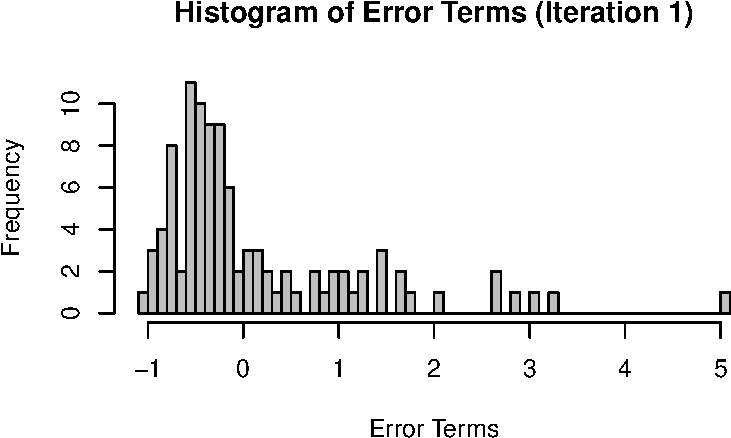
\includegraphics{HW-4-CODE-and-ANSWERS_files/figure-pdf/unnamed-chunk-11-1.pdf}

\begin{Shaded}
\begin{Highlighting}[]
\CommentTok{\# Normal Quantile Plot}

\FunctionTok{qqnorm}\NormalTok{(Epsilon.skew[, }\DecValTok{1}\NormalTok{], }
       \AttributeTok{main =} \StringTok{"Normal Q{-}Q Plot of Error Terms (Iteration 1)"}\NormalTok{)}
\FunctionTok{qqline}\NormalTok{(Epsilon.skew[, }\DecValTok{1}\NormalTok{], }\AttributeTok{col =} \StringTok{"darkred"}\NormalTok{)}
\end{Highlighting}
\end{Shaded}

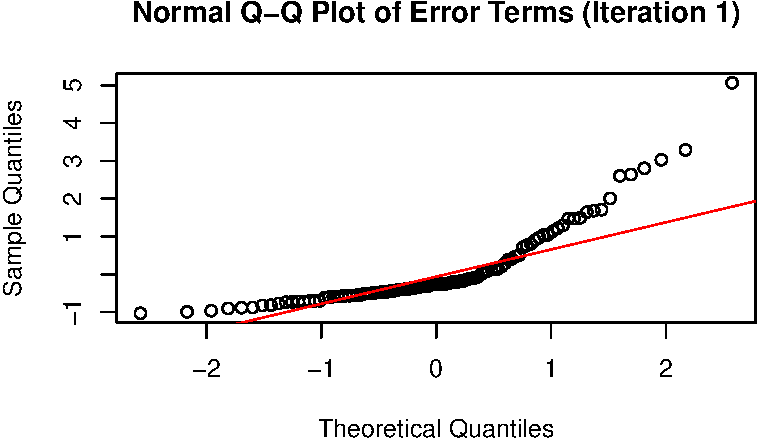
\includegraphics{HW-4-CODE-and-ANSWERS_files/figure-pdf/unnamed-chunk-11-2.pdf}

\paragraph{PART(e)}\label{parte}

\begin{Shaded}
\begin{Highlighting}[]
\CommentTok{\# Histogram of estimated slopes}
\FunctionTok{hist}\NormalTok{(b1.skew, }\AttributeTok{probability =} \ConstantTok{TRUE}\NormalTok{, }
     \AttributeTok{main =} \StringTok{"Distribution of Sample Slopes"}\NormalTok{,}
     \AttributeTok{xlab =} \StringTok{"Estimated Slope Coefficient"}\NormalTok{, }\AttributeTok{col =} \StringTok{"green"}\NormalTok{, }\AttributeTok{breaks =} \DecValTok{55}\NormalTok{)}

\CommentTok{\# Overlay normal density}
\FunctionTok{curve}\NormalTok{(}\FunctionTok{dnorm}\NormalTok{(x, }\AttributeTok{mean =} \FunctionTok{mean}\NormalTok{(b1.skew), }\AttributeTok{sd =} \FunctionTok{sd}\NormalTok{(b1.skew)), }\AttributeTok{add =} \ConstantTok{TRUE}\NormalTok{, }\AttributeTok{col =} \StringTok{"darkred"}\NormalTok{)}
\end{Highlighting}
\end{Shaded}

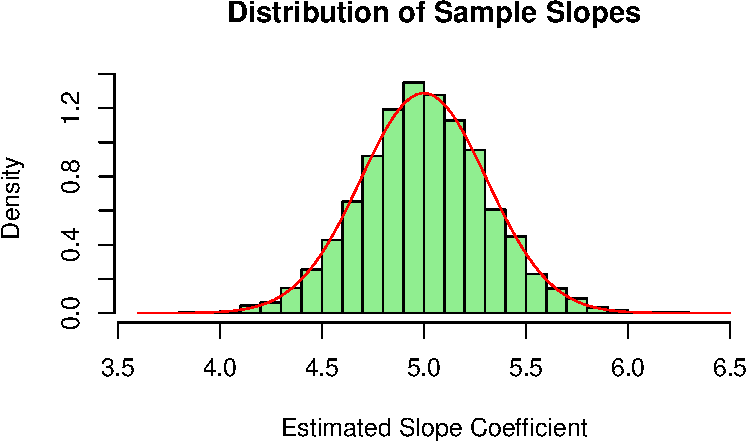
\includegraphics{HW-4-CODE-and-ANSWERS_files/figure-pdf/unnamed-chunk-12-1.pdf}

\paragraph{PART(f)}\label{partf}

\begin{Shaded}
\begin{Highlighting}[]
\CommentTok{\# Histogram for se.skew}
\FunctionTok{hist}\NormalTok{(se.skew, }
     \AttributeTok{main =} \StringTok{"Distribution of Standard Errors (Homoskedasticity)"}\NormalTok{,}
     \AttributeTok{xlab =} \StringTok{"Standard Error"}\NormalTok{, }\AttributeTok{col =} \StringTok{"coral"}\NormalTok{, }\AttributeTok{breaks =} \DecValTok{60}\NormalTok{)}
\end{Highlighting}
\end{Shaded}

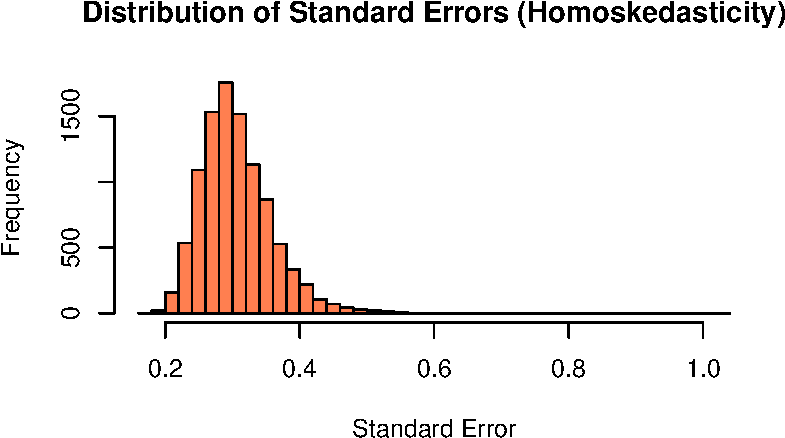
\includegraphics{HW-4-CODE-and-ANSWERS_files/figure-pdf/unnamed-chunk-13-1.pdf}

\begin{Shaded}
\begin{Highlighting}[]
\CommentTok{\# Histogram for se.skew.hc}
\FunctionTok{hist}\NormalTok{(se.skew.hc, }
     \AttributeTok{main =} \StringTok{"Distribution of Standard Errors (Heteroskedasticity Consistent)"}\NormalTok{,}
     \AttributeTok{xlab =} \StringTok{"Standard Error"}\NormalTok{, }\AttributeTok{col =} \StringTok{"yellow"}\NormalTok{, }\AttributeTok{breaks =} \DecValTok{50}\NormalTok{)}
\end{Highlighting}
\end{Shaded}

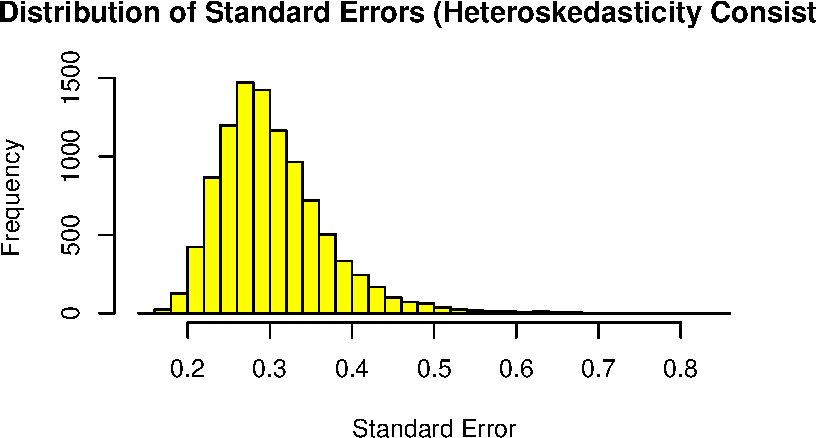
\includegraphics{HW-4-CODE-and-ANSWERS_files/figure-pdf/unnamed-chunk-13-2.pdf}

\begin{Shaded}
\begin{Highlighting}[]
\CommentTok{\# Check means}
\NormalTok{mean\_se\_skew }\OtherTok{=} \FunctionTok{mean}\NormalTok{(se.skew)}
\NormalTok{mean\_se\_skew\_hc }\OtherTok{=} \FunctionTok{mean}\NormalTok{(se.skew.hc)}

\FunctionTok{cat}\NormalTok{(}\StringTok{"Mean of se.skew:"}\NormalTok{, mean\_se\_skew, }\StringTok{"}\SpecialCharTok{\textbackslash{}n}\StringTok{"}\NormalTok{)}
\end{Highlighting}
\end{Shaded}

\begin{verbatim}
Mean of se.skew: 0.3064303 
\end{verbatim}

\begin{Shaded}
\begin{Highlighting}[]
\FunctionTok{cat}\NormalTok{(}\StringTok{"Mean of se.skew.hc:"}\NormalTok{, mean\_se\_skew\_hc, }\StringTok{"}\SpecialCharTok{\textbackslash{}n}\StringTok{"}\NormalTok{)}
\end{Highlighting}
\end{Shaded}

\begin{verbatim}
Mean of se.skew.hc: 0.303425 
\end{verbatim}

\paragraph{\texorpdfstring{\textbf{PART(g) - Confidence
Intervals}}{PART(g) - Confidence Intervals}}\label{partg---confidence-intervals}

\begin{Shaded}
\begin{Highlighting}[]
\NormalTok{true\_slope }\OtherTok{=} \DecValTok{5}

\CommentTok{\# Confidence intervals using se.skew}
\NormalTok{lower\_bound\_hom }\OtherTok{=}\NormalTok{ b1.skew }\SpecialCharTok{{-}} \FunctionTok{qt}\NormalTok{(}\FloatTok{0.975}\NormalTok{, }\AttributeTok{df =}\NormalTok{ n }\SpecialCharTok{{-}} \DecValTok{2}\NormalTok{) }\SpecialCharTok{*}\NormalTok{ se.skew}
\NormalTok{upper\_bound\_hom }\OtherTok{=}\NormalTok{ b1.skew }\SpecialCharTok{+} \FunctionTok{qt}\NormalTok{(}\FloatTok{0.975}\NormalTok{, }\AttributeTok{df =}\NormalTok{ n }\SpecialCharTok{{-}} \DecValTok{2}\NormalTok{) }\SpecialCharTok{*}\NormalTok{ se.skew}

\CommentTok{\# Confidence intervals using se.skew.hc}
\NormalTok{lower\_bound\_het }\OtherTok{=}\NormalTok{ b1.skew }\SpecialCharTok{{-}} \FunctionTok{qt}\NormalTok{(}\FloatTok{0.975}\NormalTok{, }\AttributeTok{df =}\NormalTok{ n }\SpecialCharTok{{-}} \DecValTok{2}\NormalTok{) }\SpecialCharTok{*}\NormalTok{ se.skew.hc}
\NormalTok{upper\_bound\_het }\OtherTok{=}\NormalTok{ b1.skew }\SpecialCharTok{+} \FunctionTok{qt}\NormalTok{(}\FloatTok{0.975}\NormalTok{, }\AttributeTok{df =}\NormalTok{ n }\SpecialCharTok{{-}} \DecValTok{2}\NormalTok{) }\SpecialCharTok{*}\NormalTok{ se.skew.hc}
\end{Highlighting}
\end{Shaded}

\paragraph{PART(h) - Coverage
calculation}\label{parth---coverage-calculation}

\begin{Shaded}
\begin{Highlighting}[]
\NormalTok{coverage\_hom }\OtherTok{=} \FunctionTok{mean}\NormalTok{(lower\_bound\_hom }\SpecialCharTok{\textless{}=}\NormalTok{ true\_slope }\SpecialCharTok{\&} 
\NormalTok{                      upper\_bound\_hom }\SpecialCharTok{\textgreater{}=}\NormalTok{ true\_slope)}
\NormalTok{coverage\_het }\OtherTok{=} \FunctionTok{mean}\NormalTok{(lower\_bound\_het }\SpecialCharTok{\textless{}=}\NormalTok{ true\_slope }\SpecialCharTok{\&} 
\NormalTok{                      upper\_bound\_het }\SpecialCharTok{\textgreater{}=}\NormalTok{ true\_slope)}

\FunctionTok{cat}\NormalTok{(}\StringTok{"Coverage using se.skew:"}\NormalTok{, coverage\_hom, }\StringTok{"}\SpecialCharTok{\textbackslash{}n}\StringTok{"}\NormalTok{)}
\end{Highlighting}
\end{Shaded}

\begin{verbatim}
Coverage using se.skew: 0.9508 
\end{verbatim}

\begin{Shaded}
\begin{Highlighting}[]
\FunctionTok{cat}\NormalTok{(}\StringTok{"Coverage using se.skew.hc:"}\NormalTok{, coverage\_het, }\StringTok{"}\SpecialCharTok{\textbackslash{}n}\StringTok{"}\NormalTok{)}
\end{Highlighting}
\end{Shaded}

\begin{verbatim}
Coverage using se.skew.hc: 0.952 
\end{verbatim}

\paragraph{Simulation-2 and interpretation of
results}\label{simulation-2-and-interpretation-of-results}

\begin{Shaded}
\begin{Highlighting}[]
\NormalTok{Sigma }\OtherTok{=} \FunctionTok{diag}\NormalTok{((}\FloatTok{3.6}\SpecialCharTok{*}\FunctionTok{sqrt}\NormalTok{(.}\DecValTok{75}\NormalTok{)}\SpecialCharTok{*}\FunctionTok{abs}\NormalTok{(x }\SpecialCharTok{{-}} \DecValTok{1}\SpecialCharTok{/}\DecValTok{2}\NormalTok{)))}\SpecialCharTok{\^{}}\DecValTok{2}
\NormalTok{Xmat }\OtherTok{=} \FunctionTok{cbind}\NormalTok{(}\FunctionTok{rep}\NormalTok{(}\DecValTok{1}\NormalTok{,n), x)}
\NormalTok{SD.b1.het }\OtherTok{=} \FunctionTok{sqrt}\NormalTok{((}\FunctionTok{solve}\NormalTok{(}\FunctionTok{t}\NormalTok{(Xmat)}\SpecialCharTok{\%*\%}\NormalTok{Xmat)}\SpecialCharTok{\%*\%}\FunctionTok{t}\NormalTok{(Xmat)}\SpecialCharTok{\%*\%}
\NormalTok{                    Sigma}\SpecialCharTok{\%*\%}\NormalTok{Xmat}\SpecialCharTok{\%*\%}\FunctionTok{solve}\NormalTok{(}\FunctionTok{t}\NormalTok{(Xmat)}\SpecialCharTok{\%*\%}\NormalTok{Xmat))[}\DecValTok{2}\NormalTok{,}\DecValTok{2}\NormalTok{])}

\NormalTok{nsim }\OtherTok{=} \DecValTok{10000}
\NormalTok{b1.het }\OtherTok{=} \FunctionTok{rep}\NormalTok{(}\DecValTok{0}\NormalTok{, nsim)}
\NormalTok{se.het }\OtherTok{=} \FunctionTok{rep}\NormalTok{(}\DecValTok{0}\NormalTok{, nsim)}
\NormalTok{se.het.hc }\OtherTok{=} \FunctionTok{rep}\NormalTok{(}\DecValTok{0}\NormalTok{, nsim)}
\NormalTok{Epsilon.het }\OtherTok{=} \FunctionTok{matrix}\NormalTok{(}\DecValTok{0}\NormalTok{, n, nsim)}
\ControlFlowTok{for}\NormalTok{(i }\ControlFlowTok{in} \DecValTok{1}\SpecialCharTok{:}\NormalTok{nsim)}
\NormalTok{\{}
\NormalTok{  errors }\OtherTok{=} \FunctionTok{rnorm}\NormalTok{(n, }\DecValTok{0}\NormalTok{, }\FloatTok{3.6}\SpecialCharTok{*}\FunctionTok{sqrt}\NormalTok{(.}\DecValTok{75}\NormalTok{)}\SpecialCharTok{*}\FunctionTok{abs}\NormalTok{(x }\SpecialCharTok{{-}} \DecValTok{1}\SpecialCharTok{/}\DecValTok{2}\NormalTok{))}
\NormalTok{  Y }\OtherTok{=}\NormalTok{ beta0 }\SpecialCharTok{+}\NormalTok{ beta1}\SpecialCharTok{*}\NormalTok{x }\SpecialCharTok{+}\NormalTok{ errors}
\NormalTok{  lm.temp }\OtherTok{=} \FunctionTok{lm}\NormalTok{(Y}\SpecialCharTok{\textasciitilde{}}\NormalTok{x)}
\NormalTok{  b1.het[i] }\OtherTok{=}\NormalTok{ lm.temp}\SpecialCharTok{$}\NormalTok{coef[}\DecValTok{2}\NormalTok{]}
\NormalTok{  se.het[i] }\OtherTok{=} \FunctionTok{summary}\NormalTok{(lm.temp)}\SpecialCharTok{$}\NormalTok{coef[}\DecValTok{2}\NormalTok{,}\DecValTok{2}\NormalTok{]}
\NormalTok{  se.het.hc[i] }\OtherTok{=} \FunctionTok{sqrt}\NormalTok{(}\FunctionTok{diag}\NormalTok{(}\FunctionTok{vcovHC}\NormalTok{(lm.temp, }\AttributeTok{type =} \StringTok{"HC2"}\NormalTok{)))[}\DecValTok{2}\NormalTok{]}
\NormalTok{  Epsilon.het[,i] }\OtherTok{=}\NormalTok{ errors}
\NormalTok{\}}
\end{Highlighting}
\end{Shaded}

\textbf{Some Initial Visualizations} \textbf{\& Histograms}

\begin{Shaded}
\begin{Highlighting}[]
\FunctionTok{hist}\NormalTok{(Epsilon.het[, }\DecValTok{1}\NormalTok{], }\AttributeTok{main =} \StringTok{"Histogram of Error Terms (Iteration 1)"}\NormalTok{, }
     \AttributeTok{xlab =} \StringTok{"Error Terms"}\NormalTok{, }\AttributeTok{breaks =} \DecValTok{40}\NormalTok{, }\AttributeTok{col =} \StringTok{"cyan"}\NormalTok{)}
\end{Highlighting}
\end{Shaded}

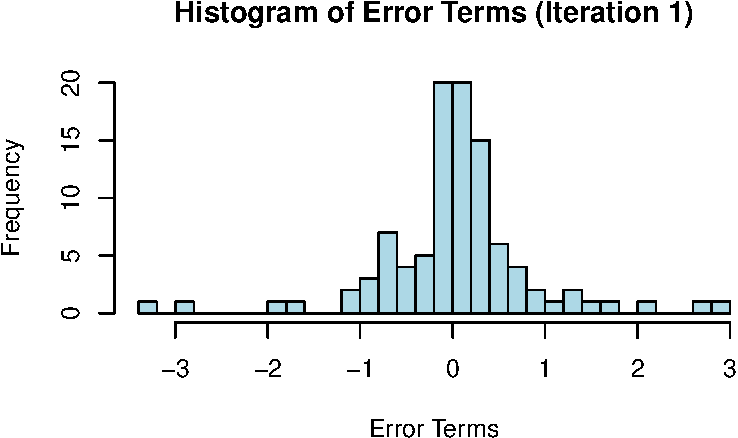
\includegraphics{HW-4-CODE-and-ANSWERS_files/figure-pdf/unnamed-chunk-17-1.pdf}

\begin{Shaded}
\begin{Highlighting}[]
\CommentTok{\# Normal Quantile Plot}
\FunctionTok{qqnorm}\NormalTok{(Epsilon.het[, }\DecValTok{1}\NormalTok{], }\AttributeTok{main =} \StringTok{"Normal Q{-}Q Plot of Error Terms (Iteration 1)"}\NormalTok{)}
\FunctionTok{qqline}\NormalTok{(Epsilon.het[, }\DecValTok{1}\NormalTok{], }\AttributeTok{col =} \StringTok{"darkred"}\NormalTok{)}
\end{Highlighting}
\end{Shaded}

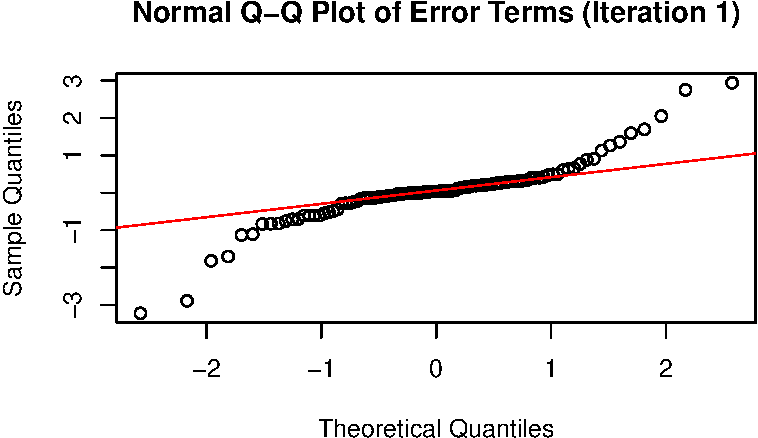
\includegraphics{HW-4-CODE-and-ANSWERS_files/figure-pdf/unnamed-chunk-17-2.pdf}

\begin{Shaded}
\begin{Highlighting}[]
\CommentTok{\# Histogram of estimated slopes}
\FunctionTok{hist}\NormalTok{(b1.het, }\AttributeTok{probability =} \ConstantTok{TRUE}\NormalTok{, }
     \AttributeTok{main =} \StringTok{"Distribution of Sample Slopes"}\NormalTok{, }
     \AttributeTok{xlab =} \StringTok{"Estimated Slope Coefficient"}\NormalTok{, }\AttributeTok{col =} \StringTok{"limegreen"}\NormalTok{, }\AttributeTok{breaks =} \DecValTok{40}\NormalTok{)}

\CommentTok{\# Overlay normal density}
\FunctionTok{curve}\NormalTok{(}\FunctionTok{dnorm}\NormalTok{(x, }\AttributeTok{mean =} \FunctionTok{mean}\NormalTok{(b1.het), }\AttributeTok{sd =} \FunctionTok{sd}\NormalTok{(b1.het)), }\AttributeTok{add =} \ConstantTok{TRUE}\NormalTok{, }\AttributeTok{col =} \StringTok{"darkred"}\NormalTok{)}
\end{Highlighting}
\end{Shaded}

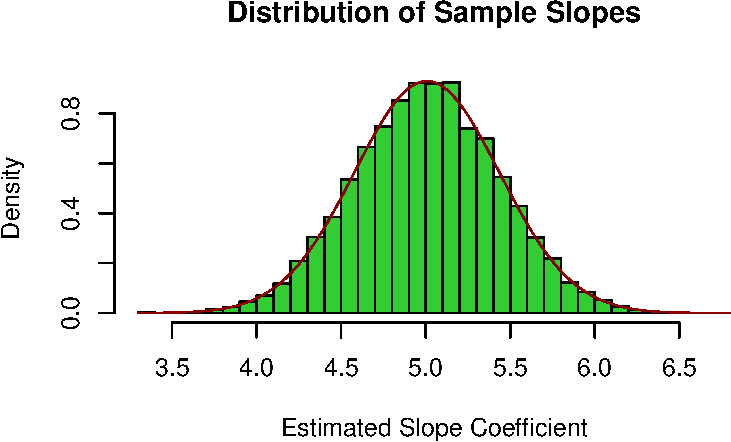
\includegraphics{HW-4-CODE-and-ANSWERS_files/figure-pdf/unnamed-chunk-17-3.pdf}

\begin{Shaded}
\begin{Highlighting}[]
\CommentTok{\# Histogram for se.het}
\FunctionTok{hist}\NormalTok{(se.het, }
     \AttributeTok{main =} \StringTok{"Distribution of Standard Errors (Homoskedasticity)"}\NormalTok{, }
     \AttributeTok{xlab =} \StringTok{"Standard Error"}\NormalTok{, }\AttributeTok{col =} \StringTok{"coral"}\NormalTok{, }\AttributeTok{breaks =} \DecValTok{40}\NormalTok{)}
\end{Highlighting}
\end{Shaded}

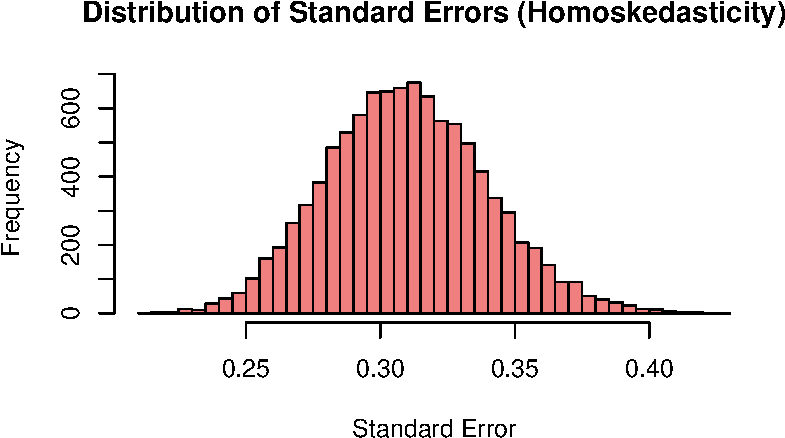
\includegraphics{HW-4-CODE-and-ANSWERS_files/figure-pdf/unnamed-chunk-17-4.pdf}

\begin{Shaded}
\begin{Highlighting}[]
\CommentTok{\# Histogram for se.het.hc}
\FunctionTok{hist}\NormalTok{(se.het.hc, }
     \AttributeTok{main =} \StringTok{"Distribution of Standard Errors (Heteroskedasticity Consistent)"}\NormalTok{, }
     \AttributeTok{xlab =} \StringTok{"Standard Error"}\NormalTok{, }\AttributeTok{col =} \StringTok{"yellow"}\NormalTok{, }\AttributeTok{breaks =} \DecValTok{40}\NormalTok{)}
\end{Highlighting}
\end{Shaded}

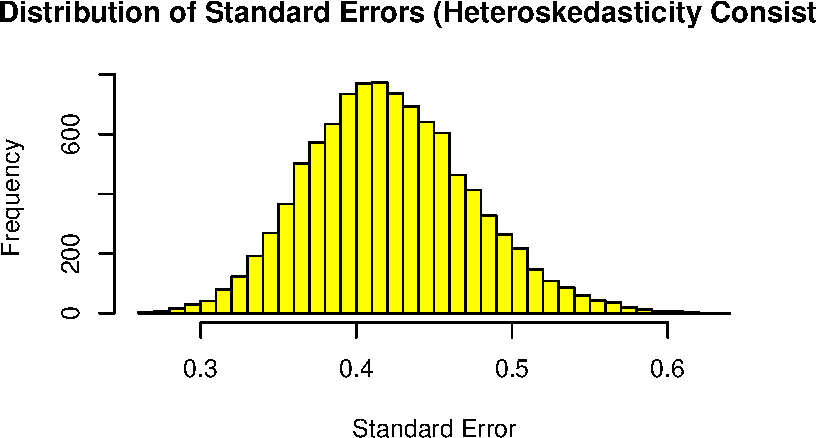
\includegraphics{HW-4-CODE-and-ANSWERS_files/figure-pdf/unnamed-chunk-17-5.pdf}

\begin{Shaded}
\begin{Highlighting}[]
\NormalTok{mean\_se\_het }\OtherTok{=} \FunctionTok{mean}\NormalTok{(se.het)}
\NormalTok{mean\_se\_het\_hc }\OtherTok{=} \FunctionTok{mean}\NormalTok{(se.het.hc)}

\FunctionTok{cat}\NormalTok{(}\StringTok{"Mean of se.het:"}\NormalTok{, mean\_se\_het, }\StringTok{"}\SpecialCharTok{\textbackslash{}n}\StringTok{"}\NormalTok{)}
\end{Highlighting}
\end{Shaded}

\begin{verbatim}
Mean of se.het: 0.3097563 
\end{verbatim}

\begin{Shaded}
\begin{Highlighting}[]
\FunctionTok{cat}\NormalTok{(}\StringTok{"Mean of se.het.hc:"}\NormalTok{, mean\_se\_het\_hc, }\StringTok{"}\SpecialCharTok{\textbackslash{}n}\StringTok{"}\NormalTok{)}
\end{Highlighting}
\end{Shaded}

\begin{verbatim}
Mean of se.het.hc: 0.4213828 
\end{verbatim}

\begin{Shaded}
\begin{Highlighting}[]
\CommentTok{\# True population slope }
\NormalTok{true\_slope }\OtherTok{=}\NormalTok{ beta1}

\CommentTok{\# Confidence intervals using se.het}
\NormalTok{lower\_bound\_hom\_het }\OtherTok{=}\NormalTok{ b1.het }\SpecialCharTok{{-}} \FunctionTok{qt}\NormalTok{(}\FloatTok{0.975}\NormalTok{, }\AttributeTok{df =}\NormalTok{ n }\SpecialCharTok{{-}} \DecValTok{2}\NormalTok{) }\SpecialCharTok{*}\NormalTok{ se.het}
\NormalTok{upper\_bound\_hom\_het }\OtherTok{=}\NormalTok{ b1.het }\SpecialCharTok{+} \FunctionTok{qt}\NormalTok{(}\FloatTok{0.975}\NormalTok{, }\AttributeTok{df =}\NormalTok{ n }\SpecialCharTok{{-}} \DecValTok{2}\NormalTok{) }\SpecialCharTok{*}\NormalTok{ se.het}

\CommentTok{\# Confidence intervals using se.het.hc}
\NormalTok{lower\_bound\_het\_hc }\OtherTok{=}\NormalTok{ b1.het }\SpecialCharTok{{-}} \FunctionTok{qt}\NormalTok{(}\FloatTok{0.975}\NormalTok{, }\AttributeTok{df =}\NormalTok{ n }\SpecialCharTok{{-}} \DecValTok{2}\NormalTok{) }\SpecialCharTok{*}\NormalTok{ se.het.hc}
\NormalTok{upper\_bound\_het\_hc }\OtherTok{=}\NormalTok{ b1.het }\SpecialCharTok{+} \FunctionTok{qt}\NormalTok{(}\FloatTok{0.975}\NormalTok{, }\AttributeTok{df =}\NormalTok{ n }\SpecialCharTok{{-}} \DecValTok{2}\NormalTok{) }\SpecialCharTok{*}\NormalTok{ se.het.hc}

\CommentTok{\# Coverage calculation}
\NormalTok{coverage\_hom\_het }\OtherTok{=} \FunctionTok{mean}\NormalTok{(lower\_bound\_hom\_het }\SpecialCharTok{\textless{}=}\NormalTok{ true\_slope }\SpecialCharTok{\&} 
\NormalTok{                          upper\_bound\_hom\_het }\SpecialCharTok{\textgreater{}=}\NormalTok{ true\_slope)}
\NormalTok{coverage\_het\_hc }\OtherTok{=} \FunctionTok{mean}\NormalTok{(lower\_bound\_het\_hc }\SpecialCharTok{\textless{}=}\NormalTok{ true\_slope }\SpecialCharTok{\&} 
\NormalTok{                         upper\_bound\_het\_hc }\SpecialCharTok{\textgreater{}=}\NormalTok{ true\_slope)}

\FunctionTok{cat}\NormalTok{(}\StringTok{"Coverage using se.het:"}\NormalTok{, coverage\_hom\_het, }\StringTok{"}\SpecialCharTok{\textbackslash{}n}\StringTok{"}\NormalTok{)}
\end{Highlighting}
\end{Shaded}

\begin{verbatim}
Coverage using se.het: 0.845 
\end{verbatim}

\begin{Shaded}
\begin{Highlighting}[]
\FunctionTok{cat}\NormalTok{(}\StringTok{"Coverage using se.het.hc:"}\NormalTok{, coverage\_het\_hc, }\StringTok{"}\SpecialCharTok{\textbackslash{}n}\StringTok{"}\NormalTok{)}
\end{Highlighting}
\end{Shaded}

\begin{verbatim}
Coverage using se.het.hc: 0.9438 
\end{verbatim}

\paragraph{PART(i)}\label{parti}

\begin{Shaded}
\begin{Highlighting}[]
\FunctionTok{plot}\NormalTok{(x, Epsilon.het[, }\DecValTok{1}\NormalTok{], }\AttributeTok{main =} \StringTok{"Scatter Plot of x vs. Epsilon (Iteration 1)"}\NormalTok{, }
     \AttributeTok{xlab =} \StringTok{"x"}\NormalTok{, }\AttributeTok{ylab =} \StringTok{"Epsilon"}\NormalTok{, }\AttributeTok{col =} \StringTok{"navy"}\NormalTok{, }\AttributeTok{pch =} \DecValTok{19}\NormalTok{, }\AttributeTok{cex=}\FloatTok{0.8}\NormalTok{)}
\end{Highlighting}
\end{Shaded}

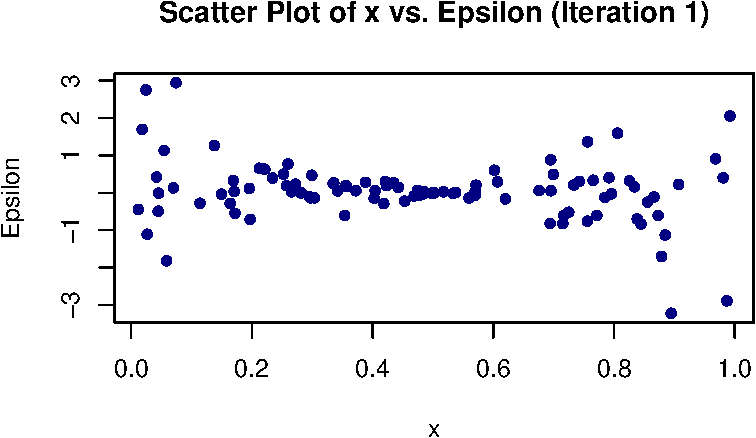
\includegraphics{HW-4-CODE-and-ANSWERS_files/figure-pdf/unnamed-chunk-18-1.pdf}

\paragraph{PART(j)}\label{partj}

\begin{Shaded}
\begin{Highlighting}[]
\FunctionTok{hist}\NormalTok{(b1.het, }\AttributeTok{probability =} \ConstantTok{TRUE}\NormalTok{, }\AttributeTok{main =} \StringTok{"Distribution of Sample Slopes"}\NormalTok{, }
     \AttributeTok{xlab =} \StringTok{"Estimated Slope Coefficient"}\NormalTok{, }\AttributeTok{col =} \StringTok{"limegreen"}\NormalTok{, }\AttributeTok{breaks =} \DecValTok{30}\NormalTok{)}

\FunctionTok{curve}\NormalTok{(}\FunctionTok{dnorm}\NormalTok{(x, }\AttributeTok{mean =} \FunctionTok{mean}\NormalTok{(b1.het), }\AttributeTok{sd =} \FunctionTok{sd}\NormalTok{(b1.het)), }\AttributeTok{add =} \ConstantTok{TRUE}\NormalTok{, }\AttributeTok{col =} \StringTok{"darkred"}\NormalTok{)}
\end{Highlighting}
\end{Shaded}

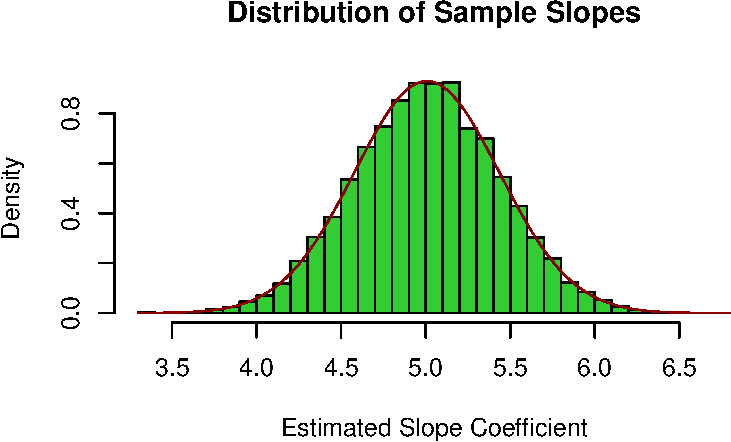
\includegraphics{HW-4-CODE-and-ANSWERS_files/figure-pdf/unnamed-chunk-19-1.pdf}

\paragraph{PART(k)}\label{partk}

\begin{Shaded}
\begin{Highlighting}[]
\FunctionTok{hist}\NormalTok{(se.het, }
     \AttributeTok{main =} \StringTok{"Distribution of Standard Errors (Homoskedasticity)"}\NormalTok{, }
     \AttributeTok{xlab =} \StringTok{"Standard Error"}\NormalTok{, }\AttributeTok{col =} \StringTok{"coral"}\NormalTok{, }\AttributeTok{breaks =} \DecValTok{40}\NormalTok{)}
\end{Highlighting}
\end{Shaded}

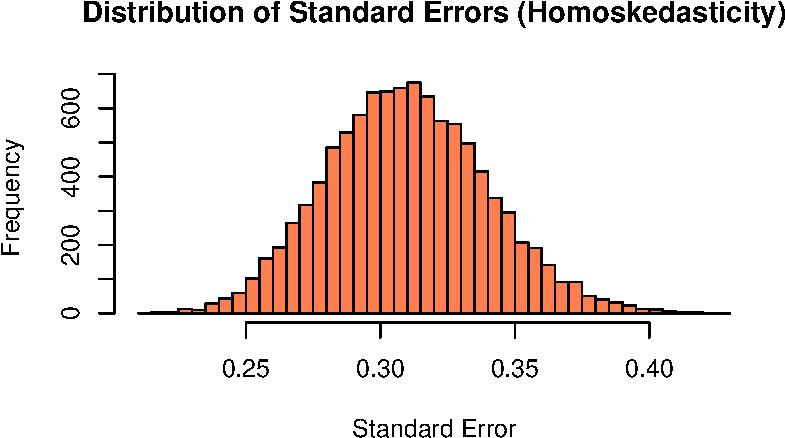
\includegraphics{HW-4-CODE-and-ANSWERS_files/figure-pdf/unnamed-chunk-20-1.pdf}

\begin{Shaded}
\begin{Highlighting}[]
\FunctionTok{hist}\NormalTok{(se.het.hc, }
     \AttributeTok{main =} \StringTok{"Distribution of Standard Errors (Heteroskedasticity Consistent)"}\NormalTok{, }
     \AttributeTok{xlab =} \StringTok{"Standard Error"}\NormalTok{, }\AttributeTok{col =} \StringTok{"yellow"}\NormalTok{, }\AttributeTok{breaks =} \DecValTok{40}\NormalTok{)}
\end{Highlighting}
\end{Shaded}

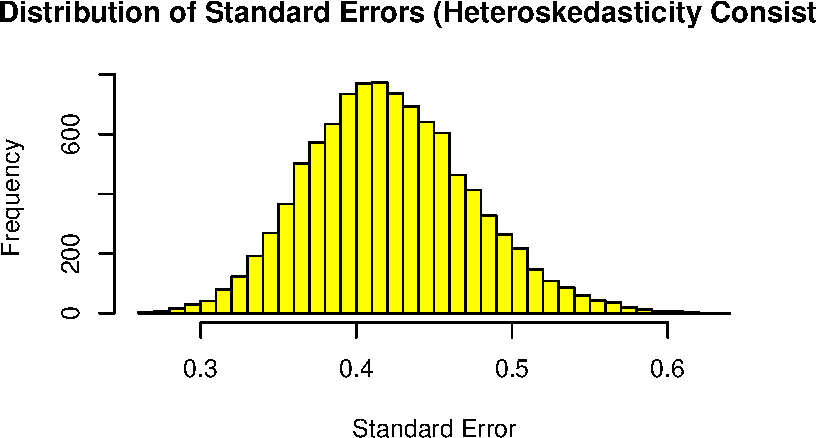
\includegraphics{HW-4-CODE-and-ANSWERS_files/figure-pdf/unnamed-chunk-20-2.pdf}

\begin{Shaded}
\begin{Highlighting}[]
\NormalTok{mean\_se\_het }\OtherTok{=} \FunctionTok{mean}\NormalTok{(se.het)}
\NormalTok{mean\_se\_het\_hc }\OtherTok{=} \FunctionTok{mean}\NormalTok{(se.het.hc)}

\FunctionTok{cat}\NormalTok{(}\StringTok{"Mean of se.het:"}\NormalTok{, mean\_se\_het, }\StringTok{"}\SpecialCharTok{\textbackslash{}n}\StringTok{"}\NormalTok{)}
\end{Highlighting}
\end{Shaded}

\begin{verbatim}
Mean of se.het: 0.3097563 
\end{verbatim}

\begin{Shaded}
\begin{Highlighting}[]
\FunctionTok{cat}\NormalTok{(}\StringTok{"Mean of se.het.hc:"}\NormalTok{, mean\_se\_het\_hc, }\StringTok{"}\SpecialCharTok{\textbackslash{}n}\StringTok{"}\NormalTok{)}
\end{Highlighting}
\end{Shaded}

\begin{verbatim}
Mean of se.het.hc: 0.4213828 
\end{verbatim}

\begin{Shaded}
\begin{Highlighting}[]
\FunctionTok{cat}\NormalTok{(}\StringTok{"True SD of beta1:"}\NormalTok{, }\FloatTok{0.427}\NormalTok{, }\StringTok{"}\SpecialCharTok{\textbackslash{}n}\StringTok{"}\NormalTok{)}
\end{Highlighting}
\end{Shaded}

\begin{verbatim}
True SD of beta1: 0.427 
\end{verbatim}

\paragraph{PART(l)}\label{partl}

\begin{Shaded}
\begin{Highlighting}[]
\NormalTok{true\_slope }\OtherTok{=} \DecValTok{5}
\NormalTok{lower\_bound\_hom\_het }\OtherTok{=}\NormalTok{ b1.het }\SpecialCharTok{{-}} \FunctionTok{qt}\NormalTok{(}\FloatTok{0.975}\NormalTok{, }\AttributeTok{df =}\NormalTok{ n }\SpecialCharTok{{-}} \DecValTok{2}\NormalTok{) }\SpecialCharTok{*}\NormalTok{ se.het}
\NormalTok{upper\_bound\_hom\_het }\OtherTok{=}\NormalTok{ b1.het }\SpecialCharTok{+} \FunctionTok{qt}\NormalTok{(}\FloatTok{0.975}\NormalTok{, }\AttributeTok{df =}\NormalTok{ n }\SpecialCharTok{{-}} \DecValTok{2}\NormalTok{) }\SpecialCharTok{*}\NormalTok{ se.het}
\NormalTok{lower\_bound\_het\_hc }\OtherTok{=}\NormalTok{ b1.het }\SpecialCharTok{{-}} \FunctionTok{qt}\NormalTok{(}\FloatTok{0.975}\NormalTok{, }\AttributeTok{df =}\NormalTok{ n }\SpecialCharTok{{-}} \DecValTok{2}\NormalTok{) }\SpecialCharTok{*}\NormalTok{ se.het.hc}
\NormalTok{upper\_bound\_het\_hc }\OtherTok{=}\NormalTok{ b1.het }\SpecialCharTok{+} \FunctionTok{qt}\NormalTok{(}\FloatTok{0.975}\NormalTok{, }\AttributeTok{df =}\NormalTok{ n }\SpecialCharTok{{-}} \DecValTok{2}\NormalTok{) }\SpecialCharTok{*}\NormalTok{ se.het.hc}
\end{Highlighting}
\end{Shaded}

\paragraph{PART(m)}\label{partm}

\begin{Shaded}
\begin{Highlighting}[]
\NormalTok{coverage\_hom\_het }\OtherTok{=} \FunctionTok{mean}\NormalTok{(lower\_bound\_hom\_het }\SpecialCharTok{\textless{}=}\NormalTok{ true\_slope }\SpecialCharTok{\&} 
\NormalTok{                          upper\_bound\_hom\_het }\SpecialCharTok{\textgreater{}=}\NormalTok{ true\_slope)}
\NormalTok{coverage\_het\_hc }\OtherTok{=} \FunctionTok{mean}\NormalTok{(lower\_bound\_het\_hc }\SpecialCharTok{\textless{}=}\NormalTok{ true\_slope }\SpecialCharTok{\&} 
\NormalTok{                         upper\_bound\_het\_hc }\SpecialCharTok{\textgreater{}=}\NormalTok{ true\_slope)}

\FunctionTok{cat}\NormalTok{(}\StringTok{"Coverage using se.het:"}\NormalTok{, coverage\_hom\_het, }\StringTok{"}\SpecialCharTok{\textbackslash{}n}\StringTok{"}\NormalTok{)}
\end{Highlighting}
\end{Shaded}

\begin{verbatim}
Coverage using se.het: 0.845 
\end{verbatim}

\begin{Shaded}
\begin{Highlighting}[]
\FunctionTok{cat}\NormalTok{(}\StringTok{"Coverage using se.het.hc:"}\NormalTok{, coverage\_het\_hc, }\StringTok{"}\SpecialCharTok{\textbackslash{}n}\StringTok{"}\NormalTok{)}
\end{Highlighting}
\end{Shaded}

\begin{verbatim}
Coverage using se.het.hc: 0.9438 
\end{verbatim}

\textbf{Results from all of the above code is discussed in attached
handwritten note.}




\end{document}
